\section{Preliminaries}
\label{sec:preliminaries}

Propositional logic satisfiability (SAT) is the problem of telling if a given formula in propositional logic is satisfiable, i.e., if there is a assignment to all involved Boolean variables that causes the whole formula to reduce to the logical value $\textit{True}$. As such, the problem occurs at every application involved complex constraints or reasoning, like (software) product lines, the tracing of software dependencies or formal methods.

It can be trivially shown that (when introducing a linear amount of new variables) all SAT problems can be reduced to a specific type of SAT problem called 3SAT, where the input propositional logic formula has to be in conjunctive normal form with all of the disjunctions containing exactly three literals.

For example, the formula $\Psi = ( x_{1} \vee x_{2} \vee x_{3}) \wedge ( \lnot x_{1} \vee x_{2} \vee x_{3})$ is in 3SAT form and is satisfiable because the assignment $(x_1 \mapsto \textit{True}, x_2 \mapsto \textit{True}, x_2 \mapsto \textit{True})$ causes the formula to reduce to $\textit{True}$. The formula $\Phi = ( x_{1} \vee x_{1} \vee x_{1}) \wedge ( \lnot x_{1} \vee \lnot x_{1}  \vee \lnot x_{1} )$ is also in 3SAT form but is not satisfiable.

\subsubsection{Definition (3SAT)}
A 3SAT instance with $m$ clauses and $n$ variables is given as a list of clauses $(c_k)_{0 \leq k \leq m-1}$ of the form $c_k = (l_{3k} \land l_{3k+1} \land l_{3k+1})$ and a list of variables $(v_j)_{0 \leq j \leq n-1}$ so that $l_i$ is a literal of the form $l_i \in \bigcup_{0 \leq j \leq n-1} \{v_j, \lnot v_j\}$. A given 3SAT instance is \emph{satisfiable} iff there exists a variable assignment $(v_j \mapsto b_j)_{0 \leq j \leq n-1}$ with $b_j \in \{\textit{True}, \textit{False}\}$ so that $\bigwedge_{0 \leq k \leq m-1} c_k$ reduces to $\textit{True}$ when interpreting all logical operators as is common. The problem of deciding whether a given 3SAT instance is satisfiable is called 3SAT.\\ \\

3SAT is of special importance to complexity theory as it was the first problem which was shown to be NP-complete \cite{cook1971complexity}. This means that every problem in NP can be reduced to 3SAT in polynomial time. It follows that any means to solve 3SAT efficiently would thus give rise to efficient solutions for any problem in NP like graph coloring, travelling salesman or bin packing.

%The K-Satisfiability Problem (hereinafter called \emph{K-SAT}) belongs to the class of NP-complete problems. K-SAT (for K $\geq$ 3) is a central problem in combinatorial optimization and was the first problem for which NP-completeness could be shown \cite{mezard2002random}.
%
%According to \cite{mezard2002random} the problem can be formulated as follows:
%Given is a set $\mathcal{B}$ consisting of N Boolean \emph{variables}. K variables are selected from the set $\mathcal{B}$ and they (or their negations) are then combined by (K-1) OR-Operators to form a \emph{clause}.
%In this way M clauses are formed. These clauses are joined by applying (M-1) AND-Operators such that a K-SAT instance is created.\\The K-SAT problem asks the question, whether there is an allocation of the boolean variables from $\mathcal{B}$, so that a given K-SAT instance can be fulfilled. 
%
%In this paper only randomly generated K-SAT instances for K = 3 are considered. These problems are then called 3-SAT and are NP-complete after \cite{cook1971complexity}.\\
%
%\textbf{Example 3-SAT instance.} \emph{As explained in the previous problem formulation, a 3-SAT instance consists of 3 variables per clause. An instance of a 3-SAT problem is for example:} $\Psi = ( x_{1} \vee x_{2} \vee x_{3}) \wedge ( \overline{x_{1}} \vee x_{2} \vee x_{3})$.\\

\subsection{Phase transitions in SAT solving}
Despite the fact that for NP-complete problems in general no algorithm is known which can solve all problem instances of a problem efficiently, i.e. in polynomial time, it is within the scope of knowledge, that certain problem instances for many NP-complete problems, including 3SAT, are easy to solve \cite{cheeseman1991really}. In \cite{monasson1999determining} this characteristic is described with a phase transition. The boundary of this phase transition divides the problem space into two regions. In one region a solution can be found relatively easily, because the solution density for these problems is high, in the other region it is very unlikely that problems can contain a correct solution at all. Problems that are very difficult to solve are located directly at this phase boundary \cite{cheeseman1991really}. 

It can be observed that, with randomly generated 3SAT instances, the probability of finding a correct solution decreases abruptly when the ratio of clauses to variables $\alpha = m/n$ exceeds a critical value of $\alpha_{c}$ \cite{monasson1996entropy}. According to \cite{mezard2002random} this critical point is $\alpha_{c} \approx $ 4.267 for randomly generated 3SAT instances. In the surrounding area of the critical point, finding a solution (i.e., deciding if the instance is satisfiable) is algorithmically complex. Figure~\ref{fig:crit_sat} illustrates this phenomenon.


\begin{figure}
	\centering
	% Created by tikzDevice version 0.12 on 2018-12-18 00:26:11
% !TEX encoding = UTF-8 Unicode
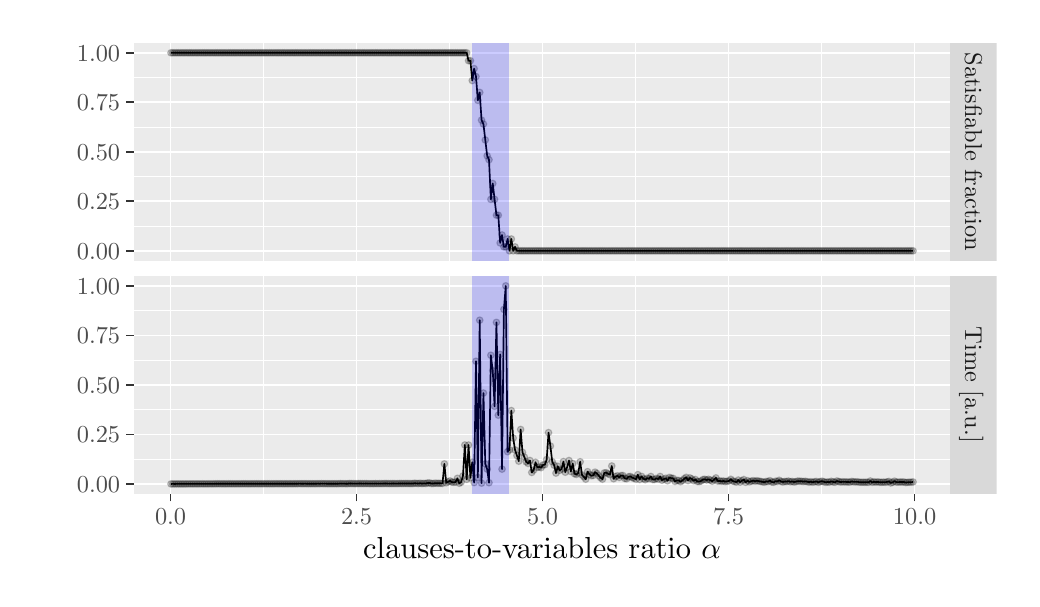
\begin{tikzpicture}[x=1pt,y=1pt]
\definecolor{fillColor}{RGB}{255,255,255}
\path[use as bounding box,fill=fillColor,fill opacity=0.00] (0,0) rectangle (355.66,199.17);
\begin{scope}
\path[clip] (  0.00,  0.00) rectangle (355.66,199.17);
\definecolor{drawColor}{RGB}{255,255,255}
\definecolor{fillColor}{RGB}{255,255,255}

\path[draw=drawColor,line width= 0.6pt,line join=round,line cap=round,fill=fillColor] (  0.00,  0.00) rectangle (355.66,199.17);
\end{scope}
\begin{scope}
\path[clip] ( 38.36,114.95) rectangle (333.35,193.67);
\definecolor{fillColor}{gray}{0.92}

\path[fill=fillColor] ( 38.36,114.95) rectangle (333.35,193.67);
\definecolor{drawColor}{RGB}{255,255,255}

\path[draw=drawColor,line width= 0.3pt,line join=round] ( 38.36,127.47) --
	(333.35,127.47);

\path[draw=drawColor,line width= 0.3pt,line join=round] ( 38.36,145.36) --
	(333.35,145.36);

\path[draw=drawColor,line width= 0.3pt,line join=round] ( 38.36,163.25) --
	(333.35,163.25);

\path[draw=drawColor,line width= 0.3pt,line join=round] ( 38.36,181.15) --
	(333.35,181.15);

\path[draw=drawColor,line width= 0.3pt,line join=round] ( 85.24,114.95) --
	( 85.24,193.67);

\path[draw=drawColor,line width= 0.3pt,line join=round] (152.45,114.95) --
	(152.45,193.67);

\path[draw=drawColor,line width= 0.3pt,line join=round] (219.67,114.95) --
	(219.67,193.67);

\path[draw=drawColor,line width= 0.3pt,line join=round] (286.88,114.95) --
	(286.88,193.67);

\path[draw=drawColor,line width= 0.6pt,line join=round] ( 38.36,118.53) --
	(333.35,118.53);

\path[draw=drawColor,line width= 0.6pt,line join=round] ( 38.36,136.42) --
	(333.35,136.42);

\path[draw=drawColor,line width= 0.6pt,line join=round] ( 38.36,154.31) --
	(333.35,154.31);

\path[draw=drawColor,line width= 0.6pt,line join=round] ( 38.36,172.20) --
	(333.35,172.20);

\path[draw=drawColor,line width= 0.6pt,line join=round] ( 38.36,190.09) --
	(333.35,190.09);

\path[draw=drawColor,line width= 0.6pt,line join=round] ( 51.64,114.95) --
	( 51.64,193.67);

\path[draw=drawColor,line width= 0.6pt,line join=round] (118.85,114.95) --
	(118.85,193.67);

\path[draw=drawColor,line width= 0.6pt,line join=round] (186.06,114.95) --
	(186.06,193.67);

\path[draw=drawColor,line width= 0.6pt,line join=round] (253.27,114.95) --
	(253.27,193.67);

\path[draw=drawColor,line width= 0.6pt,line join=round] (320.48,114.95) --
	(320.48,193.67);
\definecolor{drawColor}{RGB}{0,0,0}
\definecolor{fillColor}{RGB}{0,0,0}

\path[draw=drawColor,draw opacity=0.20,line width= 0.4pt,line join=round,line cap=round,fill=fillColor,fill opacity=0.20] ( 51.77,190.09) circle (  1.21);

\path[draw=drawColor,draw opacity=0.20,line width= 0.4pt,line join=round,line cap=round,fill=fillColor,fill opacity=0.20] ( 52.44,190.09) circle (  1.21);

\path[draw=drawColor,draw opacity=0.20,line width= 0.4pt,line join=round,line cap=round,fill=fillColor,fill opacity=0.20] ( 53.11,190.09) circle (  1.21);

\path[draw=drawColor,draw opacity=0.20,line width= 0.4pt,line join=round,line cap=round,fill=fillColor,fill opacity=0.20] ( 53.79,190.09) circle (  1.21);

\path[draw=drawColor,draw opacity=0.20,line width= 0.4pt,line join=round,line cap=round,fill=fillColor,fill opacity=0.20] ( 54.46,190.09) circle (  1.21);

\path[draw=drawColor,draw opacity=0.20,line width= 0.4pt,line join=round,line cap=round,fill=fillColor,fill opacity=0.20] ( 55.13,190.09) circle (  1.21);

\path[draw=drawColor,draw opacity=0.20,line width= 0.4pt,line join=round,line cap=round,fill=fillColor,fill opacity=0.20] ( 55.80,190.09) circle (  1.21);

\path[draw=drawColor,draw opacity=0.20,line width= 0.4pt,line join=round,line cap=round,fill=fillColor,fill opacity=0.20] ( 56.47,190.09) circle (  1.21);

\path[draw=drawColor,draw opacity=0.20,line width= 0.4pt,line join=round,line cap=round,fill=fillColor,fill opacity=0.20] ( 57.15,190.09) circle (  1.21);

\path[draw=drawColor,draw opacity=0.20,line width= 0.4pt,line join=round,line cap=round,fill=fillColor,fill opacity=0.20] ( 57.82,190.09) circle (  1.21);

\path[draw=drawColor,draw opacity=0.20,line width= 0.4pt,line join=round,line cap=round,fill=fillColor,fill opacity=0.20] ( 58.49,190.09) circle (  1.21);

\path[draw=drawColor,draw opacity=0.20,line width= 0.4pt,line join=round,line cap=round,fill=fillColor,fill opacity=0.20] ( 59.16,190.09) circle (  1.21);

\path[draw=drawColor,draw opacity=0.20,line width= 0.4pt,line join=round,line cap=round,fill=fillColor,fill opacity=0.20] ( 59.83,190.09) circle (  1.21);

\path[draw=drawColor,draw opacity=0.20,line width= 0.4pt,line join=round,line cap=round,fill=fillColor,fill opacity=0.20] ( 60.51,190.09) circle (  1.21);

\path[draw=drawColor,draw opacity=0.20,line width= 0.4pt,line join=round,line cap=round,fill=fillColor,fill opacity=0.20] ( 61.18,190.09) circle (  1.21);

\path[draw=drawColor,draw opacity=0.20,line width= 0.4pt,line join=round,line cap=round,fill=fillColor,fill opacity=0.20] ( 61.85,190.09) circle (  1.21);

\path[draw=drawColor,draw opacity=0.20,line width= 0.4pt,line join=round,line cap=round,fill=fillColor,fill opacity=0.20] ( 62.52,190.09) circle (  1.21);

\path[draw=drawColor,draw opacity=0.20,line width= 0.4pt,line join=round,line cap=round,fill=fillColor,fill opacity=0.20] ( 63.20,190.09) circle (  1.21);

\path[draw=drawColor,draw opacity=0.20,line width= 0.4pt,line join=round,line cap=round,fill=fillColor,fill opacity=0.20] ( 63.87,190.09) circle (  1.21);

\path[draw=drawColor,draw opacity=0.20,line width= 0.4pt,line join=round,line cap=round,fill=fillColor,fill opacity=0.20] ( 64.54,190.09) circle (  1.21);

\path[draw=drawColor,draw opacity=0.20,line width= 0.4pt,line join=round,line cap=round,fill=fillColor,fill opacity=0.20] ( 65.21,190.09) circle (  1.21);

\path[draw=drawColor,draw opacity=0.20,line width= 0.4pt,line join=round,line cap=round,fill=fillColor,fill opacity=0.20] ( 65.88,190.09) circle (  1.21);

\path[draw=drawColor,draw opacity=0.20,line width= 0.4pt,line join=round,line cap=round,fill=fillColor,fill opacity=0.20] ( 66.56,190.09) circle (  1.21);

\path[draw=drawColor,draw opacity=0.20,line width= 0.4pt,line join=round,line cap=round,fill=fillColor,fill opacity=0.20] ( 67.23,190.09) circle (  1.21);

\path[draw=drawColor,draw opacity=0.20,line width= 0.4pt,line join=round,line cap=round,fill=fillColor,fill opacity=0.20] ( 67.90,190.09) circle (  1.21);

\path[draw=drawColor,draw opacity=0.20,line width= 0.4pt,line join=round,line cap=round,fill=fillColor,fill opacity=0.20] ( 68.57,190.09) circle (  1.21);

\path[draw=drawColor,draw opacity=0.20,line width= 0.4pt,line join=round,line cap=round,fill=fillColor,fill opacity=0.20] ( 69.24,190.09) circle (  1.21);

\path[draw=drawColor,draw opacity=0.20,line width= 0.4pt,line join=round,line cap=round,fill=fillColor,fill opacity=0.20] ( 69.92,190.09) circle (  1.21);

\path[draw=drawColor,draw opacity=0.20,line width= 0.4pt,line join=round,line cap=round,fill=fillColor,fill opacity=0.20] ( 70.59,190.09) circle (  1.21);

\path[draw=drawColor,draw opacity=0.20,line width= 0.4pt,line join=round,line cap=round,fill=fillColor,fill opacity=0.20] ( 71.26,190.09) circle (  1.21);

\path[draw=drawColor,draw opacity=0.20,line width= 0.4pt,line join=round,line cap=round,fill=fillColor,fill opacity=0.20] ( 71.93,190.09) circle (  1.21);

\path[draw=drawColor,draw opacity=0.20,line width= 0.4pt,line join=round,line cap=round,fill=fillColor,fill opacity=0.20] ( 72.61,190.09) circle (  1.21);

\path[draw=drawColor,draw opacity=0.20,line width= 0.4pt,line join=round,line cap=round,fill=fillColor,fill opacity=0.20] ( 73.28,190.09) circle (  1.21);

\path[draw=drawColor,draw opacity=0.20,line width= 0.4pt,line join=round,line cap=round,fill=fillColor,fill opacity=0.20] ( 73.95,190.09) circle (  1.21);

\path[draw=drawColor,draw opacity=0.20,line width= 0.4pt,line join=round,line cap=round,fill=fillColor,fill opacity=0.20] ( 74.62,190.09) circle (  1.21);

\path[draw=drawColor,draw opacity=0.20,line width= 0.4pt,line join=round,line cap=round,fill=fillColor,fill opacity=0.20] ( 75.29,190.09) circle (  1.21);

\path[draw=drawColor,draw opacity=0.20,line width= 0.4pt,line join=round,line cap=round,fill=fillColor,fill opacity=0.20] ( 75.97,190.09) circle (  1.21);

\path[draw=drawColor,draw opacity=0.20,line width= 0.4pt,line join=round,line cap=round,fill=fillColor,fill opacity=0.20] ( 76.64,190.09) circle (  1.21);

\path[draw=drawColor,draw opacity=0.20,line width= 0.4pt,line join=round,line cap=round,fill=fillColor,fill opacity=0.20] ( 77.31,190.09) circle (  1.21);

\path[draw=drawColor,draw opacity=0.20,line width= 0.4pt,line join=round,line cap=round,fill=fillColor,fill opacity=0.20] ( 77.98,190.09) circle (  1.21);

\path[draw=drawColor,draw opacity=0.20,line width= 0.4pt,line join=round,line cap=round,fill=fillColor,fill opacity=0.20] ( 78.65,190.09) circle (  1.21);

\path[draw=drawColor,draw opacity=0.20,line width= 0.4pt,line join=round,line cap=round,fill=fillColor,fill opacity=0.20] ( 79.33,190.09) circle (  1.21);

\path[draw=drawColor,draw opacity=0.20,line width= 0.4pt,line join=round,line cap=round,fill=fillColor,fill opacity=0.20] ( 80.00,190.09) circle (  1.21);

\path[draw=drawColor,draw opacity=0.20,line width= 0.4pt,line join=round,line cap=round,fill=fillColor,fill opacity=0.20] ( 80.67,190.09) circle (  1.21);

\path[draw=drawColor,draw opacity=0.20,line width= 0.4pt,line join=round,line cap=round,fill=fillColor,fill opacity=0.20] ( 81.34,190.09) circle (  1.21);

\path[draw=drawColor,draw opacity=0.20,line width= 0.4pt,line join=round,line cap=round,fill=fillColor,fill opacity=0.20] ( 82.01,190.09) circle (  1.21);

\path[draw=drawColor,draw opacity=0.20,line width= 0.4pt,line join=round,line cap=round,fill=fillColor,fill opacity=0.20] ( 82.69,190.09) circle (  1.21);

\path[draw=drawColor,draw opacity=0.20,line width= 0.4pt,line join=round,line cap=round,fill=fillColor,fill opacity=0.20] ( 83.36,190.09) circle (  1.21);

\path[draw=drawColor,draw opacity=0.20,line width= 0.4pt,line join=round,line cap=round,fill=fillColor,fill opacity=0.20] ( 84.03,190.09) circle (  1.21);

\path[draw=drawColor,draw opacity=0.20,line width= 0.4pt,line join=round,line cap=round,fill=fillColor,fill opacity=0.20] ( 84.70,190.09) circle (  1.21);

\path[draw=drawColor,draw opacity=0.20,line width= 0.4pt,line join=round,line cap=round,fill=fillColor,fill opacity=0.20] ( 85.38,190.09) circle (  1.21);

\path[draw=drawColor,draw opacity=0.20,line width= 0.4pt,line join=round,line cap=round,fill=fillColor,fill opacity=0.20] ( 86.05,190.09) circle (  1.21);

\path[draw=drawColor,draw opacity=0.20,line width= 0.4pt,line join=round,line cap=round,fill=fillColor,fill opacity=0.20] ( 86.72,190.09) circle (  1.21);

\path[draw=drawColor,draw opacity=0.20,line width= 0.4pt,line join=round,line cap=round,fill=fillColor,fill opacity=0.20] ( 87.39,190.09) circle (  1.21);

\path[draw=drawColor,draw opacity=0.20,line width= 0.4pt,line join=round,line cap=round,fill=fillColor,fill opacity=0.20] ( 88.06,190.09) circle (  1.21);

\path[draw=drawColor,draw opacity=0.20,line width= 0.4pt,line join=round,line cap=round,fill=fillColor,fill opacity=0.20] ( 88.74,190.09) circle (  1.21);

\path[draw=drawColor,draw opacity=0.20,line width= 0.4pt,line join=round,line cap=round,fill=fillColor,fill opacity=0.20] ( 89.41,190.09) circle (  1.21);

\path[draw=drawColor,draw opacity=0.20,line width= 0.4pt,line join=round,line cap=round,fill=fillColor,fill opacity=0.20] ( 90.08,190.09) circle (  1.21);

\path[draw=drawColor,draw opacity=0.20,line width= 0.4pt,line join=round,line cap=round,fill=fillColor,fill opacity=0.20] ( 90.75,190.09) circle (  1.21);

\path[draw=drawColor,draw opacity=0.20,line width= 0.4pt,line join=round,line cap=round,fill=fillColor,fill opacity=0.20] ( 91.42,190.09) circle (  1.21);

\path[draw=drawColor,draw opacity=0.20,line width= 0.4pt,line join=round,line cap=round,fill=fillColor,fill opacity=0.20] ( 92.10,190.09) circle (  1.21);

\path[draw=drawColor,draw opacity=0.20,line width= 0.4pt,line join=round,line cap=round,fill=fillColor,fill opacity=0.20] ( 92.77,190.09) circle (  1.21);

\path[draw=drawColor,draw opacity=0.20,line width= 0.4pt,line join=round,line cap=round,fill=fillColor,fill opacity=0.20] ( 93.44,190.09) circle (  1.21);

\path[draw=drawColor,draw opacity=0.20,line width= 0.4pt,line join=round,line cap=round,fill=fillColor,fill opacity=0.20] ( 94.11,190.09) circle (  1.21);

\path[draw=drawColor,draw opacity=0.20,line width= 0.4pt,line join=round,line cap=round,fill=fillColor,fill opacity=0.20] ( 94.79,190.09) circle (  1.21);

\path[draw=drawColor,draw opacity=0.20,line width= 0.4pt,line join=round,line cap=round,fill=fillColor,fill opacity=0.20] ( 95.46,190.09) circle (  1.21);

\path[draw=drawColor,draw opacity=0.20,line width= 0.4pt,line join=round,line cap=round,fill=fillColor,fill opacity=0.20] ( 96.13,190.09) circle (  1.21);

\path[draw=drawColor,draw opacity=0.20,line width= 0.4pt,line join=round,line cap=round,fill=fillColor,fill opacity=0.20] ( 96.80,190.09) circle (  1.21);

\path[draw=drawColor,draw opacity=0.20,line width= 0.4pt,line join=round,line cap=round,fill=fillColor,fill opacity=0.20] ( 97.47,190.09) circle (  1.21);

\path[draw=drawColor,draw opacity=0.20,line width= 0.4pt,line join=round,line cap=round,fill=fillColor,fill opacity=0.20] ( 98.15,190.09) circle (  1.21);

\path[draw=drawColor,draw opacity=0.20,line width= 0.4pt,line join=round,line cap=round,fill=fillColor,fill opacity=0.20] ( 98.82,190.09) circle (  1.21);

\path[draw=drawColor,draw opacity=0.20,line width= 0.4pt,line join=round,line cap=round,fill=fillColor,fill opacity=0.20] ( 99.49,190.09) circle (  1.21);

\path[draw=drawColor,draw opacity=0.20,line width= 0.4pt,line join=round,line cap=round,fill=fillColor,fill opacity=0.20] (100.16,190.09) circle (  1.21);

\path[draw=drawColor,draw opacity=0.20,line width= 0.4pt,line join=round,line cap=round,fill=fillColor,fill opacity=0.20] (100.83,190.09) circle (  1.21);

\path[draw=drawColor,draw opacity=0.20,line width= 0.4pt,line join=round,line cap=round,fill=fillColor,fill opacity=0.20] (101.51,190.09) circle (  1.21);

\path[draw=drawColor,draw opacity=0.20,line width= 0.4pt,line join=round,line cap=round,fill=fillColor,fill opacity=0.20] (102.18,190.09) circle (  1.21);

\path[draw=drawColor,draw opacity=0.20,line width= 0.4pt,line join=round,line cap=round,fill=fillColor,fill opacity=0.20] (102.85,190.09) circle (  1.21);

\path[draw=drawColor,draw opacity=0.20,line width= 0.4pt,line join=round,line cap=round,fill=fillColor,fill opacity=0.20] (103.52,190.09) circle (  1.21);

\path[draw=drawColor,draw opacity=0.20,line width= 0.4pt,line join=round,line cap=round,fill=fillColor,fill opacity=0.20] (104.19,190.09) circle (  1.21);

\path[draw=drawColor,draw opacity=0.20,line width= 0.4pt,line join=round,line cap=round,fill=fillColor,fill opacity=0.20] (104.87,190.09) circle (  1.21);

\path[draw=drawColor,draw opacity=0.20,line width= 0.4pt,line join=round,line cap=round,fill=fillColor,fill opacity=0.20] (105.54,190.09) circle (  1.21);

\path[draw=drawColor,draw opacity=0.20,line width= 0.4pt,line join=round,line cap=round,fill=fillColor,fill opacity=0.20] (106.21,190.09) circle (  1.21);

\path[draw=drawColor,draw opacity=0.20,line width= 0.4pt,line join=round,line cap=round,fill=fillColor,fill opacity=0.20] (106.88,190.09) circle (  1.21);

\path[draw=drawColor,draw opacity=0.20,line width= 0.4pt,line join=round,line cap=round,fill=fillColor,fill opacity=0.20] (107.56,190.09) circle (  1.21);

\path[draw=drawColor,draw opacity=0.20,line width= 0.4pt,line join=round,line cap=round,fill=fillColor,fill opacity=0.20] (108.23,190.09) circle (  1.21);

\path[draw=drawColor,draw opacity=0.20,line width= 0.4pt,line join=round,line cap=round,fill=fillColor,fill opacity=0.20] (108.90,190.09) circle (  1.21);

\path[draw=drawColor,draw opacity=0.20,line width= 0.4pt,line join=round,line cap=round,fill=fillColor,fill opacity=0.20] (109.57,190.09) circle (  1.21);

\path[draw=drawColor,draw opacity=0.20,line width= 0.4pt,line join=round,line cap=round,fill=fillColor,fill opacity=0.20] (110.24,190.09) circle (  1.21);

\path[draw=drawColor,draw opacity=0.20,line width= 0.4pt,line join=round,line cap=round,fill=fillColor,fill opacity=0.20] (110.92,190.09) circle (  1.21);

\path[draw=drawColor,draw opacity=0.20,line width= 0.4pt,line join=round,line cap=round,fill=fillColor,fill opacity=0.20] (111.59,190.09) circle (  1.21);

\path[draw=drawColor,draw opacity=0.20,line width= 0.4pt,line join=round,line cap=round,fill=fillColor,fill opacity=0.20] (112.26,190.09) circle (  1.21);

\path[draw=drawColor,draw opacity=0.20,line width= 0.4pt,line join=round,line cap=round,fill=fillColor,fill opacity=0.20] (112.93,190.09) circle (  1.21);

\path[draw=drawColor,draw opacity=0.20,line width= 0.4pt,line join=round,line cap=round,fill=fillColor,fill opacity=0.20] (113.60,190.09) circle (  1.21);

\path[draw=drawColor,draw opacity=0.20,line width= 0.4pt,line join=round,line cap=round,fill=fillColor,fill opacity=0.20] (114.28,190.09) circle (  1.21);

\path[draw=drawColor,draw opacity=0.20,line width= 0.4pt,line join=round,line cap=round,fill=fillColor,fill opacity=0.20] (114.95,190.09) circle (  1.21);

\path[draw=drawColor,draw opacity=0.20,line width= 0.4pt,line join=round,line cap=round,fill=fillColor,fill opacity=0.20] (115.62,190.09) circle (  1.21);

\path[draw=drawColor,draw opacity=0.20,line width= 0.4pt,line join=round,line cap=round,fill=fillColor,fill opacity=0.20] (116.29,190.09) circle (  1.21);

\path[draw=drawColor,draw opacity=0.20,line width= 0.4pt,line join=round,line cap=round,fill=fillColor,fill opacity=0.20] (116.97,190.09) circle (  1.21);

\path[draw=drawColor,draw opacity=0.20,line width= 0.4pt,line join=round,line cap=round,fill=fillColor,fill opacity=0.20] (117.64,190.09) circle (  1.21);

\path[draw=drawColor,draw opacity=0.20,line width= 0.4pt,line join=round,line cap=round,fill=fillColor,fill opacity=0.20] (118.31,190.09) circle (  1.21);

\path[draw=drawColor,draw opacity=0.20,line width= 0.4pt,line join=round,line cap=round,fill=fillColor,fill opacity=0.20] (118.98,190.09) circle (  1.21);

\path[draw=drawColor,draw opacity=0.20,line width= 0.4pt,line join=round,line cap=round,fill=fillColor,fill opacity=0.20] (119.65,190.09) circle (  1.21);

\path[draw=drawColor,draw opacity=0.20,line width= 0.4pt,line join=round,line cap=round,fill=fillColor,fill opacity=0.20] (120.33,190.09) circle (  1.21);

\path[draw=drawColor,draw opacity=0.20,line width= 0.4pt,line join=round,line cap=round,fill=fillColor,fill opacity=0.20] (121.00,190.09) circle (  1.21);

\path[draw=drawColor,draw opacity=0.20,line width= 0.4pt,line join=round,line cap=round,fill=fillColor,fill opacity=0.20] (121.67,190.09) circle (  1.21);

\path[draw=drawColor,draw opacity=0.20,line width= 0.4pt,line join=round,line cap=round,fill=fillColor,fill opacity=0.20] (122.34,190.09) circle (  1.21);

\path[draw=drawColor,draw opacity=0.20,line width= 0.4pt,line join=round,line cap=round,fill=fillColor,fill opacity=0.20] (123.01,190.09) circle (  1.21);

\path[draw=drawColor,draw opacity=0.20,line width= 0.4pt,line join=round,line cap=round,fill=fillColor,fill opacity=0.20] (123.69,190.09) circle (  1.21);

\path[draw=drawColor,draw opacity=0.20,line width= 0.4pt,line join=round,line cap=round,fill=fillColor,fill opacity=0.20] (124.36,190.09) circle (  1.21);

\path[draw=drawColor,draw opacity=0.20,line width= 0.4pt,line join=round,line cap=round,fill=fillColor,fill opacity=0.20] (125.03,190.09) circle (  1.21);

\path[draw=drawColor,draw opacity=0.20,line width= 0.4pt,line join=round,line cap=round,fill=fillColor,fill opacity=0.20] (125.70,190.09) circle (  1.21);

\path[draw=drawColor,draw opacity=0.20,line width= 0.4pt,line join=round,line cap=round,fill=fillColor,fill opacity=0.20] (126.37,190.09) circle (  1.21);

\path[draw=drawColor,draw opacity=0.20,line width= 0.4pt,line join=round,line cap=round,fill=fillColor,fill opacity=0.20] (127.05,190.09) circle (  1.21);

\path[draw=drawColor,draw opacity=0.20,line width= 0.4pt,line join=round,line cap=round,fill=fillColor,fill opacity=0.20] (127.72,190.09) circle (  1.21);

\path[draw=drawColor,draw opacity=0.20,line width= 0.4pt,line join=round,line cap=round,fill=fillColor,fill opacity=0.20] (128.39,190.09) circle (  1.21);

\path[draw=drawColor,draw opacity=0.20,line width= 0.4pt,line join=round,line cap=round,fill=fillColor,fill opacity=0.20] (129.06,190.09) circle (  1.21);

\path[draw=drawColor,draw opacity=0.20,line width= 0.4pt,line join=round,line cap=round,fill=fillColor,fill opacity=0.20] (129.74,190.09) circle (  1.21);

\path[draw=drawColor,draw opacity=0.20,line width= 0.4pt,line join=round,line cap=round,fill=fillColor,fill opacity=0.20] (130.41,190.09) circle (  1.21);

\path[draw=drawColor,draw opacity=0.20,line width= 0.4pt,line join=round,line cap=round,fill=fillColor,fill opacity=0.20] (131.08,190.09) circle (  1.21);

\path[draw=drawColor,draw opacity=0.20,line width= 0.4pt,line join=round,line cap=round,fill=fillColor,fill opacity=0.20] (131.75,190.09) circle (  1.21);

\path[draw=drawColor,draw opacity=0.20,line width= 0.4pt,line join=round,line cap=round,fill=fillColor,fill opacity=0.20] (132.42,190.09) circle (  1.21);

\path[draw=drawColor,draw opacity=0.20,line width= 0.4pt,line join=round,line cap=round,fill=fillColor,fill opacity=0.20] (133.10,190.09) circle (  1.21);

\path[draw=drawColor,draw opacity=0.20,line width= 0.4pt,line join=round,line cap=round,fill=fillColor,fill opacity=0.20] (133.77,190.09) circle (  1.21);

\path[draw=drawColor,draw opacity=0.20,line width= 0.4pt,line join=round,line cap=round,fill=fillColor,fill opacity=0.20] (134.44,190.09) circle (  1.21);

\path[draw=drawColor,draw opacity=0.20,line width= 0.4pt,line join=round,line cap=round,fill=fillColor,fill opacity=0.20] (135.11,190.09) circle (  1.21);

\path[draw=drawColor,draw opacity=0.20,line width= 0.4pt,line join=round,line cap=round,fill=fillColor,fill opacity=0.20] (135.78,190.09) circle (  1.21);

\path[draw=drawColor,draw opacity=0.20,line width= 0.4pt,line join=round,line cap=round,fill=fillColor,fill opacity=0.20] (136.46,190.09) circle (  1.21);

\path[draw=drawColor,draw opacity=0.20,line width= 0.4pt,line join=round,line cap=round,fill=fillColor,fill opacity=0.20] (137.13,190.09) circle (  1.21);

\path[draw=drawColor,draw opacity=0.20,line width= 0.4pt,line join=round,line cap=round,fill=fillColor,fill opacity=0.20] (137.80,190.09) circle (  1.21);

\path[draw=drawColor,draw opacity=0.20,line width= 0.4pt,line join=round,line cap=round,fill=fillColor,fill opacity=0.20] (138.47,190.09) circle (  1.21);

\path[draw=drawColor,draw opacity=0.20,line width= 0.4pt,line join=round,line cap=round,fill=fillColor,fill opacity=0.20] (139.15,190.09) circle (  1.21);

\path[draw=drawColor,draw opacity=0.20,line width= 0.4pt,line join=round,line cap=round,fill=fillColor,fill opacity=0.20] (139.82,190.09) circle (  1.21);

\path[draw=drawColor,draw opacity=0.20,line width= 0.4pt,line join=round,line cap=round,fill=fillColor,fill opacity=0.20] (140.49,190.09) circle (  1.21);

\path[draw=drawColor,draw opacity=0.20,line width= 0.4pt,line join=round,line cap=round,fill=fillColor,fill opacity=0.20] (141.16,190.09) circle (  1.21);

\path[draw=drawColor,draw opacity=0.20,line width= 0.4pt,line join=round,line cap=round,fill=fillColor,fill opacity=0.20] (141.83,190.09) circle (  1.21);

\path[draw=drawColor,draw opacity=0.20,line width= 0.4pt,line join=round,line cap=round,fill=fillColor,fill opacity=0.20] (142.51,190.09) circle (  1.21);

\path[draw=drawColor,draw opacity=0.20,line width= 0.4pt,line join=round,line cap=round,fill=fillColor,fill opacity=0.20] (143.18,190.09) circle (  1.21);

\path[draw=drawColor,draw opacity=0.20,line width= 0.4pt,line join=round,line cap=round,fill=fillColor,fill opacity=0.20] (143.85,190.09) circle (  1.21);

\path[draw=drawColor,draw opacity=0.20,line width= 0.4pt,line join=round,line cap=round,fill=fillColor,fill opacity=0.20] (144.52,190.09) circle (  1.21);

\path[draw=drawColor,draw opacity=0.20,line width= 0.4pt,line join=round,line cap=round,fill=fillColor,fill opacity=0.20] (145.19,190.09) circle (  1.21);

\path[draw=drawColor,draw opacity=0.20,line width= 0.4pt,line join=round,line cap=round,fill=fillColor,fill opacity=0.20] (145.87,190.09) circle (  1.21);

\path[draw=drawColor,draw opacity=0.20,line width= 0.4pt,line join=round,line cap=round,fill=fillColor,fill opacity=0.20] (146.54,190.09) circle (  1.21);

\path[draw=drawColor,draw opacity=0.20,line width= 0.4pt,line join=round,line cap=round,fill=fillColor,fill opacity=0.20] (147.21,190.09) circle (  1.21);

\path[draw=drawColor,draw opacity=0.20,line width= 0.4pt,line join=round,line cap=round,fill=fillColor,fill opacity=0.20] (147.88,190.09) circle (  1.21);

\path[draw=drawColor,draw opacity=0.20,line width= 0.4pt,line join=round,line cap=round,fill=fillColor,fill opacity=0.20] (148.55,190.09) circle (  1.21);

\path[draw=drawColor,draw opacity=0.20,line width= 0.4pt,line join=round,line cap=round,fill=fillColor,fill opacity=0.20] (149.23,190.09) circle (  1.21);

\path[draw=drawColor,draw opacity=0.20,line width= 0.4pt,line join=round,line cap=round,fill=fillColor,fill opacity=0.20] (149.90,190.09) circle (  1.21);

\path[draw=drawColor,draw opacity=0.20,line width= 0.4pt,line join=round,line cap=round,fill=fillColor,fill opacity=0.20] (150.57,190.09) circle (  1.21);

\path[draw=drawColor,draw opacity=0.20,line width= 0.4pt,line join=round,line cap=round,fill=fillColor,fill opacity=0.20] (151.24,190.09) circle (  1.21);

\path[draw=drawColor,draw opacity=0.20,line width= 0.4pt,line join=round,line cap=round,fill=fillColor,fill opacity=0.20] (151.92,190.09) circle (  1.21);

\path[draw=drawColor,draw opacity=0.20,line width= 0.4pt,line join=round,line cap=round,fill=fillColor,fill opacity=0.20] (152.59,190.09) circle (  1.21);

\path[draw=drawColor,draw opacity=0.20,line width= 0.4pt,line join=round,line cap=round,fill=fillColor,fill opacity=0.20] (153.26,190.09) circle (  1.21);

\path[draw=drawColor,draw opacity=0.20,line width= 0.4pt,line join=round,line cap=round,fill=fillColor,fill opacity=0.20] (153.93,190.09) circle (  1.21);

\path[draw=drawColor,draw opacity=0.20,line width= 0.4pt,line join=round,line cap=round,fill=fillColor,fill opacity=0.20] (154.60,190.09) circle (  1.21);

\path[draw=drawColor,draw opacity=0.20,line width= 0.4pt,line join=round,line cap=round,fill=fillColor,fill opacity=0.20] (155.28,190.09) circle (  1.21);

\path[draw=drawColor,draw opacity=0.20,line width= 0.4pt,line join=round,line cap=round,fill=fillColor,fill opacity=0.20] (155.95,190.09) circle (  1.21);

\path[draw=drawColor,draw opacity=0.20,line width= 0.4pt,line join=round,line cap=round,fill=fillColor,fill opacity=0.20] (156.62,190.09) circle (  1.21);

\path[draw=drawColor,draw opacity=0.20,line width= 0.4pt,line join=round,line cap=round,fill=fillColor,fill opacity=0.20] (157.29,190.09) circle (  1.21);

\path[draw=drawColor,draw opacity=0.20,line width= 0.4pt,line join=round,line cap=round,fill=fillColor,fill opacity=0.20] (157.96,190.09) circle (  1.21);

\path[draw=drawColor,draw opacity=0.20,line width= 0.4pt,line join=round,line cap=round,fill=fillColor,fill opacity=0.20] (158.64,190.09) circle (  1.21);

\path[draw=drawColor,draw opacity=0.20,line width= 0.4pt,line join=round,line cap=round,fill=fillColor,fill opacity=0.20] (159.31,187.23) circle (  1.21);

\path[draw=drawColor,draw opacity=0.20,line width= 0.4pt,line join=round,line cap=round,fill=fillColor,fill opacity=0.20] (159.98,187.23) circle (  1.21);

\path[draw=drawColor,draw opacity=0.20,line width= 0.4pt,line join=round,line cap=round,fill=fillColor,fill opacity=0.20] (160.65,180.07) circle (  1.21);

\path[draw=drawColor,draw opacity=0.20,line width= 0.4pt,line join=round,line cap=round,fill=fillColor,fill opacity=0.20] (161.33,184.37) circle (  1.21);

\path[draw=drawColor,draw opacity=0.20,line width= 0.4pt,line join=round,line cap=round,fill=fillColor,fill opacity=0.20] (162.00,181.50) circle (  1.21);

\path[draw=drawColor,draw opacity=0.20,line width= 0.4pt,line join=round,line cap=round,fill=fillColor,fill opacity=0.20] (162.67,172.92) circle (  1.21);

\path[draw=drawColor,draw opacity=0.20,line width= 0.4pt,line join=round,line cap=round,fill=fillColor,fill opacity=0.20] (163.34,175.78) circle (  1.21);

\path[draw=drawColor,draw opacity=0.20,line width= 0.4pt,line join=round,line cap=round,fill=fillColor,fill opacity=0.20] (164.01,165.76) circle (  1.21);

\path[draw=drawColor,draw opacity=0.20,line width= 0.4pt,line join=round,line cap=round,fill=fillColor,fill opacity=0.20] (164.69,164.33) circle (  1.21);

\path[draw=drawColor,draw opacity=0.20,line width= 0.4pt,line join=round,line cap=round,fill=fillColor,fill opacity=0.20] (165.36,158.60) circle (  1.21);

\path[draw=drawColor,draw opacity=0.20,line width= 0.4pt,line join=round,line cap=round,fill=fillColor,fill opacity=0.20] (166.03,152.88) circle (  1.21);

\path[draw=drawColor,draw opacity=0.20,line width= 0.4pt,line join=round,line cap=round,fill=fillColor,fill opacity=0.20] (166.70,151.45) circle (  1.21);

\path[draw=drawColor,draw opacity=0.20,line width= 0.4pt,line join=round,line cap=round,fill=fillColor,fill opacity=0.20] (167.37,137.13) circle (  1.21);

\path[draw=drawColor,draw opacity=0.20,line width= 0.4pt,line join=round,line cap=round,fill=fillColor,fill opacity=0.20] (168.05,142.86) circle (  1.21);

\path[draw=drawColor,draw opacity=0.20,line width= 0.4pt,line join=round,line cap=round,fill=fillColor,fill opacity=0.20] (168.72,137.13) circle (  1.21);

\path[draw=drawColor,draw opacity=0.20,line width= 0.4pt,line join=round,line cap=round,fill=fillColor,fill opacity=0.20] (169.39,131.41) circle (  1.21);

\path[draw=drawColor,draw opacity=0.20,line width= 0.4pt,line join=round,line cap=round,fill=fillColor,fill opacity=0.20] (170.06,131.41) circle (  1.21);

\path[draw=drawColor,draw opacity=0.20,line width= 0.4pt,line join=round,line cap=round,fill=fillColor,fill opacity=0.20] (170.73,121.39) circle (  1.21);

\path[draw=drawColor,draw opacity=0.20,line width= 0.4pt,line join=round,line cap=round,fill=fillColor,fill opacity=0.20] (171.41,124.25) circle (  1.21);

\path[draw=drawColor,draw opacity=0.20,line width= 0.4pt,line join=round,line cap=round,fill=fillColor,fill opacity=0.20] (172.08,119.96) circle (  1.21);

\path[draw=drawColor,draw opacity=0.20,line width= 0.4pt,line join=round,line cap=round,fill=fillColor,fill opacity=0.20] (172.75,119.96) circle (  1.21);

\path[draw=drawColor,draw opacity=0.20,line width= 0.4pt,line join=round,line cap=round,fill=fillColor,fill opacity=0.20] (173.42,122.82) circle (  1.21);

\path[draw=drawColor,draw opacity=0.20,line width= 0.4pt,line join=round,line cap=round,fill=fillColor,fill opacity=0.20] (174.10,118.53) circle (  1.21);

\path[draw=drawColor,draw opacity=0.20,line width= 0.4pt,line join=round,line cap=round,fill=fillColor,fill opacity=0.20] (174.77,122.82) circle (  1.21);

\path[draw=drawColor,draw opacity=0.20,line width= 0.4pt,line join=round,line cap=round,fill=fillColor,fill opacity=0.20] (175.44,118.53) circle (  1.21);

\path[draw=drawColor,draw opacity=0.20,line width= 0.4pt,line join=round,line cap=round,fill=fillColor,fill opacity=0.20] (176.11,119.96) circle (  1.21);

\path[draw=drawColor,draw opacity=0.20,line width= 0.4pt,line join=round,line cap=round,fill=fillColor,fill opacity=0.20] (176.78,118.53) circle (  1.21);

\path[draw=drawColor,draw opacity=0.20,line width= 0.4pt,line join=round,line cap=round,fill=fillColor,fill opacity=0.20] (177.46,118.53) circle (  1.21);

\path[draw=drawColor,draw opacity=0.20,line width= 0.4pt,line join=round,line cap=round,fill=fillColor,fill opacity=0.20] (178.13,118.53) circle (  1.21);

\path[draw=drawColor,draw opacity=0.20,line width= 0.4pt,line join=round,line cap=round,fill=fillColor,fill opacity=0.20] (178.80,118.53) circle (  1.21);

\path[draw=drawColor,draw opacity=0.20,line width= 0.4pt,line join=round,line cap=round,fill=fillColor,fill opacity=0.20] (179.47,118.53) circle (  1.21);

\path[draw=drawColor,draw opacity=0.20,line width= 0.4pt,line join=round,line cap=round,fill=fillColor,fill opacity=0.20] (180.14,118.53) circle (  1.21);

\path[draw=drawColor,draw opacity=0.20,line width= 0.4pt,line join=round,line cap=round,fill=fillColor,fill opacity=0.20] (180.82,118.53) circle (  1.21);

\path[draw=drawColor,draw opacity=0.20,line width= 0.4pt,line join=round,line cap=round,fill=fillColor,fill opacity=0.20] (181.49,118.53) circle (  1.21);

\path[draw=drawColor,draw opacity=0.20,line width= 0.4pt,line join=round,line cap=round,fill=fillColor,fill opacity=0.20] (182.16,118.53) circle (  1.21);

\path[draw=drawColor,draw opacity=0.20,line width= 0.4pt,line join=round,line cap=round,fill=fillColor,fill opacity=0.20] (182.83,118.53) circle (  1.21);

\path[draw=drawColor,draw opacity=0.20,line width= 0.4pt,line join=round,line cap=round,fill=fillColor,fill opacity=0.20] (183.51,118.53) circle (  1.21);

\path[draw=drawColor,draw opacity=0.20,line width= 0.4pt,line join=round,line cap=round,fill=fillColor,fill opacity=0.20] (184.18,118.53) circle (  1.21);

\path[draw=drawColor,draw opacity=0.20,line width= 0.4pt,line join=round,line cap=round,fill=fillColor,fill opacity=0.20] (184.85,118.53) circle (  1.21);

\path[draw=drawColor,draw opacity=0.20,line width= 0.4pt,line join=round,line cap=round,fill=fillColor,fill opacity=0.20] (185.52,118.53) circle (  1.21);

\path[draw=drawColor,draw opacity=0.20,line width= 0.4pt,line join=round,line cap=round,fill=fillColor,fill opacity=0.20] (186.19,118.53) circle (  1.21);

\path[draw=drawColor,draw opacity=0.20,line width= 0.4pt,line join=round,line cap=round,fill=fillColor,fill opacity=0.20] (186.87,118.53) circle (  1.21);

\path[draw=drawColor,draw opacity=0.20,line width= 0.4pt,line join=round,line cap=round,fill=fillColor,fill opacity=0.20] (187.54,118.53) circle (  1.21);

\path[draw=drawColor,draw opacity=0.20,line width= 0.4pt,line join=round,line cap=round,fill=fillColor,fill opacity=0.20] (188.21,118.53) circle (  1.21);

\path[draw=drawColor,draw opacity=0.20,line width= 0.4pt,line join=round,line cap=round,fill=fillColor,fill opacity=0.20] (188.88,118.53) circle (  1.21);

\path[draw=drawColor,draw opacity=0.20,line width= 0.4pt,line join=round,line cap=round,fill=fillColor,fill opacity=0.20] (189.55,118.53) circle (  1.21);

\path[draw=drawColor,draw opacity=0.20,line width= 0.4pt,line join=round,line cap=round,fill=fillColor,fill opacity=0.20] (190.23,118.53) circle (  1.21);

\path[draw=drawColor,draw opacity=0.20,line width= 0.4pt,line join=round,line cap=round,fill=fillColor,fill opacity=0.20] (190.90,118.53) circle (  1.21);

\path[draw=drawColor,draw opacity=0.20,line width= 0.4pt,line join=round,line cap=round,fill=fillColor,fill opacity=0.20] (191.57,118.53) circle (  1.21);

\path[draw=drawColor,draw opacity=0.20,line width= 0.4pt,line join=round,line cap=round,fill=fillColor,fill opacity=0.20] (192.24,118.53) circle (  1.21);

\path[draw=drawColor,draw opacity=0.20,line width= 0.4pt,line join=round,line cap=round,fill=fillColor,fill opacity=0.20] (192.91,118.53) circle (  1.21);

\path[draw=drawColor,draw opacity=0.20,line width= 0.4pt,line join=round,line cap=round,fill=fillColor,fill opacity=0.20] (193.59,118.53) circle (  1.21);

\path[draw=drawColor,draw opacity=0.20,line width= 0.4pt,line join=round,line cap=round,fill=fillColor,fill opacity=0.20] (194.26,118.53) circle (  1.21);

\path[draw=drawColor,draw opacity=0.20,line width= 0.4pt,line join=round,line cap=round,fill=fillColor,fill opacity=0.20] (194.93,118.53) circle (  1.21);

\path[draw=drawColor,draw opacity=0.20,line width= 0.4pt,line join=round,line cap=round,fill=fillColor,fill opacity=0.20] (195.60,118.53) circle (  1.21);

\path[draw=drawColor,draw opacity=0.20,line width= 0.4pt,line join=round,line cap=round,fill=fillColor,fill opacity=0.20] (196.28,118.53) circle (  1.21);

\path[draw=drawColor,draw opacity=0.20,line width= 0.4pt,line join=round,line cap=round,fill=fillColor,fill opacity=0.20] (196.95,118.53) circle (  1.21);

\path[draw=drawColor,draw opacity=0.20,line width= 0.4pt,line join=round,line cap=round,fill=fillColor,fill opacity=0.20] (197.62,118.53) circle (  1.21);

\path[draw=drawColor,draw opacity=0.20,line width= 0.4pt,line join=round,line cap=round,fill=fillColor,fill opacity=0.20] (198.29,118.53) circle (  1.21);

\path[draw=drawColor,draw opacity=0.20,line width= 0.4pt,line join=round,line cap=round,fill=fillColor,fill opacity=0.20] (198.96,118.53) circle (  1.21);

\path[draw=drawColor,draw opacity=0.20,line width= 0.4pt,line join=round,line cap=round,fill=fillColor,fill opacity=0.20] (199.64,118.53) circle (  1.21);

\path[draw=drawColor,draw opacity=0.20,line width= 0.4pt,line join=round,line cap=round,fill=fillColor,fill opacity=0.20] (200.31,118.53) circle (  1.21);

\path[draw=drawColor,draw opacity=0.20,line width= 0.4pt,line join=round,line cap=round,fill=fillColor,fill opacity=0.20] (200.98,118.53) circle (  1.21);

\path[draw=drawColor,draw opacity=0.20,line width= 0.4pt,line join=round,line cap=round,fill=fillColor,fill opacity=0.20] (201.65,118.53) circle (  1.21);

\path[draw=drawColor,draw opacity=0.20,line width= 0.4pt,line join=round,line cap=round,fill=fillColor,fill opacity=0.20] (202.32,118.53) circle (  1.21);

\path[draw=drawColor,draw opacity=0.20,line width= 0.4pt,line join=round,line cap=round,fill=fillColor,fill opacity=0.20] (203.00,118.53) circle (  1.21);

\path[draw=drawColor,draw opacity=0.20,line width= 0.4pt,line join=round,line cap=round,fill=fillColor,fill opacity=0.20] (203.67,118.53) circle (  1.21);

\path[draw=drawColor,draw opacity=0.20,line width= 0.4pt,line join=round,line cap=round,fill=fillColor,fill opacity=0.20] (204.34,118.53) circle (  1.21);

\path[draw=drawColor,draw opacity=0.20,line width= 0.4pt,line join=round,line cap=round,fill=fillColor,fill opacity=0.20] (205.01,118.53) circle (  1.21);

\path[draw=drawColor,draw opacity=0.20,line width= 0.4pt,line join=round,line cap=round,fill=fillColor,fill opacity=0.20] (205.69,118.53) circle (  1.21);

\path[draw=drawColor,draw opacity=0.20,line width= 0.4pt,line join=round,line cap=round,fill=fillColor,fill opacity=0.20] (206.36,118.53) circle (  1.21);

\path[draw=drawColor,draw opacity=0.20,line width= 0.4pt,line join=round,line cap=round,fill=fillColor,fill opacity=0.20] (207.03,118.53) circle (  1.21);

\path[draw=drawColor,draw opacity=0.20,line width= 0.4pt,line join=round,line cap=round,fill=fillColor,fill opacity=0.20] (207.70,118.53) circle (  1.21);

\path[draw=drawColor,draw opacity=0.20,line width= 0.4pt,line join=round,line cap=round,fill=fillColor,fill opacity=0.20] (208.37,118.53) circle (  1.21);

\path[draw=drawColor,draw opacity=0.20,line width= 0.4pt,line join=round,line cap=round,fill=fillColor,fill opacity=0.20] (209.05,118.53) circle (  1.21);

\path[draw=drawColor,draw opacity=0.20,line width= 0.4pt,line join=round,line cap=round,fill=fillColor,fill opacity=0.20] (209.72,118.53) circle (  1.21);

\path[draw=drawColor,draw opacity=0.20,line width= 0.4pt,line join=round,line cap=round,fill=fillColor,fill opacity=0.20] (210.39,118.53) circle (  1.21);

\path[draw=drawColor,draw opacity=0.20,line width= 0.4pt,line join=round,line cap=round,fill=fillColor,fill opacity=0.20] (211.06,118.53) circle (  1.21);

\path[draw=drawColor,draw opacity=0.20,line width= 0.4pt,line join=round,line cap=round,fill=fillColor,fill opacity=0.20] (211.73,118.53) circle (  1.21);

\path[draw=drawColor,draw opacity=0.20,line width= 0.4pt,line join=round,line cap=round,fill=fillColor,fill opacity=0.20] (212.41,118.53) circle (  1.21);

\path[draw=drawColor,draw opacity=0.20,line width= 0.4pt,line join=round,line cap=round,fill=fillColor,fill opacity=0.20] (213.08,118.53) circle (  1.21);

\path[draw=drawColor,draw opacity=0.20,line width= 0.4pt,line join=round,line cap=round,fill=fillColor,fill opacity=0.20] (213.75,118.53) circle (  1.21);

\path[draw=drawColor,draw opacity=0.20,line width= 0.4pt,line join=round,line cap=round,fill=fillColor,fill opacity=0.20] (214.42,118.53) circle (  1.21);

\path[draw=drawColor,draw opacity=0.20,line width= 0.4pt,line join=round,line cap=round,fill=fillColor,fill opacity=0.20] (215.09,118.53) circle (  1.21);

\path[draw=drawColor,draw opacity=0.20,line width= 0.4pt,line join=round,line cap=round,fill=fillColor,fill opacity=0.20] (215.77,118.53) circle (  1.21);

\path[draw=drawColor,draw opacity=0.20,line width= 0.4pt,line join=round,line cap=round,fill=fillColor,fill opacity=0.20] (216.44,118.53) circle (  1.21);

\path[draw=drawColor,draw opacity=0.20,line width= 0.4pt,line join=round,line cap=round,fill=fillColor,fill opacity=0.20] (217.11,118.53) circle (  1.21);

\path[draw=drawColor,draw opacity=0.20,line width= 0.4pt,line join=round,line cap=round,fill=fillColor,fill opacity=0.20] (217.78,118.53) circle (  1.21);

\path[draw=drawColor,draw opacity=0.20,line width= 0.4pt,line join=round,line cap=round,fill=fillColor,fill opacity=0.20] (218.46,118.53) circle (  1.21);

\path[draw=drawColor,draw opacity=0.20,line width= 0.4pt,line join=round,line cap=round,fill=fillColor,fill opacity=0.20] (219.13,118.53) circle (  1.21);

\path[draw=drawColor,draw opacity=0.20,line width= 0.4pt,line join=round,line cap=round,fill=fillColor,fill opacity=0.20] (219.80,118.53) circle (  1.21);

\path[draw=drawColor,draw opacity=0.20,line width= 0.4pt,line join=round,line cap=round,fill=fillColor,fill opacity=0.20] (220.47,118.53) circle (  1.21);

\path[draw=drawColor,draw opacity=0.20,line width= 0.4pt,line join=round,line cap=round,fill=fillColor,fill opacity=0.20] (221.14,118.53) circle (  1.21);

\path[draw=drawColor,draw opacity=0.20,line width= 0.4pt,line join=round,line cap=round,fill=fillColor,fill opacity=0.20] (221.82,118.53) circle (  1.21);

\path[draw=drawColor,draw opacity=0.20,line width= 0.4pt,line join=round,line cap=round,fill=fillColor,fill opacity=0.20] (222.49,118.53) circle (  1.21);

\path[draw=drawColor,draw opacity=0.20,line width= 0.4pt,line join=round,line cap=round,fill=fillColor,fill opacity=0.20] (223.16,118.53) circle (  1.21);

\path[draw=drawColor,draw opacity=0.20,line width= 0.4pt,line join=round,line cap=round,fill=fillColor,fill opacity=0.20] (223.83,118.53) circle (  1.21);

\path[draw=drawColor,draw opacity=0.20,line width= 0.4pt,line join=round,line cap=round,fill=fillColor,fill opacity=0.20] (224.50,118.53) circle (  1.21);

\path[draw=drawColor,draw opacity=0.20,line width= 0.4pt,line join=round,line cap=round,fill=fillColor,fill opacity=0.20] (225.18,118.53) circle (  1.21);

\path[draw=drawColor,draw opacity=0.20,line width= 0.4pt,line join=round,line cap=round,fill=fillColor,fill opacity=0.20] (225.85,118.53) circle (  1.21);

\path[draw=drawColor,draw opacity=0.20,line width= 0.4pt,line join=round,line cap=round,fill=fillColor,fill opacity=0.20] (226.52,118.53) circle (  1.21);

\path[draw=drawColor,draw opacity=0.20,line width= 0.4pt,line join=round,line cap=round,fill=fillColor,fill opacity=0.20] (227.19,118.53) circle (  1.21);

\path[draw=drawColor,draw opacity=0.20,line width= 0.4pt,line join=round,line cap=round,fill=fillColor,fill opacity=0.20] (227.87,118.53) circle (  1.21);

\path[draw=drawColor,draw opacity=0.20,line width= 0.4pt,line join=round,line cap=round,fill=fillColor,fill opacity=0.20] (228.54,118.53) circle (  1.21);

\path[draw=drawColor,draw opacity=0.20,line width= 0.4pt,line join=round,line cap=round,fill=fillColor,fill opacity=0.20] (229.21,118.53) circle (  1.21);

\path[draw=drawColor,draw opacity=0.20,line width= 0.4pt,line join=round,line cap=round,fill=fillColor,fill opacity=0.20] (229.88,118.53) circle (  1.21);

\path[draw=drawColor,draw opacity=0.20,line width= 0.4pt,line join=round,line cap=round,fill=fillColor,fill opacity=0.20] (230.55,118.53) circle (  1.21);

\path[draw=drawColor,draw opacity=0.20,line width= 0.4pt,line join=round,line cap=round,fill=fillColor,fill opacity=0.20] (231.23,118.53) circle (  1.21);

\path[draw=drawColor,draw opacity=0.20,line width= 0.4pt,line join=round,line cap=round,fill=fillColor,fill opacity=0.20] (231.90,118.53) circle (  1.21);

\path[draw=drawColor,draw opacity=0.20,line width= 0.4pt,line join=round,line cap=round,fill=fillColor,fill opacity=0.20] (232.57,118.53) circle (  1.21);

\path[draw=drawColor,draw opacity=0.20,line width= 0.4pt,line join=round,line cap=round,fill=fillColor,fill opacity=0.20] (233.24,118.53) circle (  1.21);

\path[draw=drawColor,draw opacity=0.20,line width= 0.4pt,line join=round,line cap=round,fill=fillColor,fill opacity=0.20] (233.91,118.53) circle (  1.21);

\path[draw=drawColor,draw opacity=0.20,line width= 0.4pt,line join=round,line cap=round,fill=fillColor,fill opacity=0.20] (234.59,118.53) circle (  1.21);

\path[draw=drawColor,draw opacity=0.20,line width= 0.4pt,line join=round,line cap=round,fill=fillColor,fill opacity=0.20] (235.26,118.53) circle (  1.21);

\path[draw=drawColor,draw opacity=0.20,line width= 0.4pt,line join=round,line cap=round,fill=fillColor,fill opacity=0.20] (235.93,118.53) circle (  1.21);

\path[draw=drawColor,draw opacity=0.20,line width= 0.4pt,line join=round,line cap=round,fill=fillColor,fill opacity=0.20] (236.60,118.53) circle (  1.21);

\path[draw=drawColor,draw opacity=0.20,line width= 0.4pt,line join=round,line cap=round,fill=fillColor,fill opacity=0.20] (237.27,118.53) circle (  1.21);

\path[draw=drawColor,draw opacity=0.20,line width= 0.4pt,line join=round,line cap=round,fill=fillColor,fill opacity=0.20] (237.95,118.53) circle (  1.21);

\path[draw=drawColor,draw opacity=0.20,line width= 0.4pt,line join=round,line cap=round,fill=fillColor,fill opacity=0.20] (238.62,118.53) circle (  1.21);

\path[draw=drawColor,draw opacity=0.20,line width= 0.4pt,line join=round,line cap=round,fill=fillColor,fill opacity=0.20] (239.29,118.53) circle (  1.21);

\path[draw=drawColor,draw opacity=0.20,line width= 0.4pt,line join=round,line cap=round,fill=fillColor,fill opacity=0.20] (239.96,118.53) circle (  1.21);

\path[draw=drawColor,draw opacity=0.20,line width= 0.4pt,line join=round,line cap=round,fill=fillColor,fill opacity=0.20] (240.64,118.53) circle (  1.21);

\path[draw=drawColor,draw opacity=0.20,line width= 0.4pt,line join=round,line cap=round,fill=fillColor,fill opacity=0.20] (241.31,118.53) circle (  1.21);

\path[draw=drawColor,draw opacity=0.20,line width= 0.4pt,line join=round,line cap=round,fill=fillColor,fill opacity=0.20] (241.98,118.53) circle (  1.21);

\path[draw=drawColor,draw opacity=0.20,line width= 0.4pt,line join=round,line cap=round,fill=fillColor,fill opacity=0.20] (242.65,118.53) circle (  1.21);

\path[draw=drawColor,draw opacity=0.20,line width= 0.4pt,line join=round,line cap=round,fill=fillColor,fill opacity=0.20] (243.32,118.53) circle (  1.21);

\path[draw=drawColor,draw opacity=0.20,line width= 0.4pt,line join=round,line cap=round,fill=fillColor,fill opacity=0.20] (244.00,118.53) circle (  1.21);

\path[draw=drawColor,draw opacity=0.20,line width= 0.4pt,line join=round,line cap=round,fill=fillColor,fill opacity=0.20] (244.67,118.53) circle (  1.21);

\path[draw=drawColor,draw opacity=0.20,line width= 0.4pt,line join=round,line cap=round,fill=fillColor,fill opacity=0.20] (245.34,118.53) circle (  1.21);

\path[draw=drawColor,draw opacity=0.20,line width= 0.4pt,line join=round,line cap=round,fill=fillColor,fill opacity=0.20] (246.01,118.53) circle (  1.21);

\path[draw=drawColor,draw opacity=0.20,line width= 0.4pt,line join=round,line cap=round,fill=fillColor,fill opacity=0.20] (246.68,118.53) circle (  1.21);

\path[draw=drawColor,draw opacity=0.20,line width= 0.4pt,line join=round,line cap=round,fill=fillColor,fill opacity=0.20] (247.36,118.53) circle (  1.21);

\path[draw=drawColor,draw opacity=0.20,line width= 0.4pt,line join=round,line cap=round,fill=fillColor,fill opacity=0.20] (248.03,118.53) circle (  1.21);

\path[draw=drawColor,draw opacity=0.20,line width= 0.4pt,line join=round,line cap=round,fill=fillColor,fill opacity=0.20] (248.70,118.53) circle (  1.21);

\path[draw=drawColor,draw opacity=0.20,line width= 0.4pt,line join=round,line cap=round,fill=fillColor,fill opacity=0.20] (249.37,118.53) circle (  1.21);

\path[draw=drawColor,draw opacity=0.20,line width= 0.4pt,line join=round,line cap=round,fill=fillColor,fill opacity=0.20] (250.05,118.53) circle (  1.21);

\path[draw=drawColor,draw opacity=0.20,line width= 0.4pt,line join=round,line cap=round,fill=fillColor,fill opacity=0.20] (250.72,118.53) circle (  1.21);

\path[draw=drawColor,draw opacity=0.20,line width= 0.4pt,line join=round,line cap=round,fill=fillColor,fill opacity=0.20] (251.39,118.53) circle (  1.21);

\path[draw=drawColor,draw opacity=0.20,line width= 0.4pt,line join=round,line cap=round,fill=fillColor,fill opacity=0.20] (252.06,118.53) circle (  1.21);

\path[draw=drawColor,draw opacity=0.20,line width= 0.4pt,line join=round,line cap=round,fill=fillColor,fill opacity=0.20] (252.73,118.53) circle (  1.21);

\path[draw=drawColor,draw opacity=0.20,line width= 0.4pt,line join=round,line cap=round,fill=fillColor,fill opacity=0.20] (253.41,118.53) circle (  1.21);

\path[draw=drawColor,draw opacity=0.20,line width= 0.4pt,line join=round,line cap=round,fill=fillColor,fill opacity=0.20] (254.08,118.53) circle (  1.21);

\path[draw=drawColor,draw opacity=0.20,line width= 0.4pt,line join=round,line cap=round,fill=fillColor,fill opacity=0.20] (254.75,118.53) circle (  1.21);

\path[draw=drawColor,draw opacity=0.20,line width= 0.4pt,line join=round,line cap=round,fill=fillColor,fill opacity=0.20] (255.42,118.53) circle (  1.21);

\path[draw=drawColor,draw opacity=0.20,line width= 0.4pt,line join=round,line cap=round,fill=fillColor,fill opacity=0.20] (256.09,118.53) circle (  1.21);

\path[draw=drawColor,draw opacity=0.20,line width= 0.4pt,line join=round,line cap=round,fill=fillColor,fill opacity=0.20] (256.77,118.53) circle (  1.21);

\path[draw=drawColor,draw opacity=0.20,line width= 0.4pt,line join=round,line cap=round,fill=fillColor,fill opacity=0.20] (257.44,118.53) circle (  1.21);

\path[draw=drawColor,draw opacity=0.20,line width= 0.4pt,line join=round,line cap=round,fill=fillColor,fill opacity=0.20] (258.11,118.53) circle (  1.21);

\path[draw=drawColor,draw opacity=0.20,line width= 0.4pt,line join=round,line cap=round,fill=fillColor,fill opacity=0.20] (258.78,118.53) circle (  1.21);

\path[draw=drawColor,draw opacity=0.20,line width= 0.4pt,line join=round,line cap=round,fill=fillColor,fill opacity=0.20] (259.45,118.53) circle (  1.21);

\path[draw=drawColor,draw opacity=0.20,line width= 0.4pt,line join=round,line cap=round,fill=fillColor,fill opacity=0.20] (260.13,118.53) circle (  1.21);

\path[draw=drawColor,draw opacity=0.20,line width= 0.4pt,line join=round,line cap=round,fill=fillColor,fill opacity=0.20] (260.80,118.53) circle (  1.21);

\path[draw=drawColor,draw opacity=0.20,line width= 0.4pt,line join=round,line cap=round,fill=fillColor,fill opacity=0.20] (261.47,118.53) circle (  1.21);

\path[draw=drawColor,draw opacity=0.20,line width= 0.4pt,line join=round,line cap=round,fill=fillColor,fill opacity=0.20] (262.14,118.53) circle (  1.21);

\path[draw=drawColor,draw opacity=0.20,line width= 0.4pt,line join=round,line cap=round,fill=fillColor,fill opacity=0.20] (262.82,118.53) circle (  1.21);

\path[draw=drawColor,draw opacity=0.20,line width= 0.4pt,line join=round,line cap=round,fill=fillColor,fill opacity=0.20] (263.49,118.53) circle (  1.21);

\path[draw=drawColor,draw opacity=0.20,line width= 0.4pt,line join=round,line cap=round,fill=fillColor,fill opacity=0.20] (264.16,118.53) circle (  1.21);

\path[draw=drawColor,draw opacity=0.20,line width= 0.4pt,line join=round,line cap=round,fill=fillColor,fill opacity=0.20] (264.83,118.53) circle (  1.21);

\path[draw=drawColor,draw opacity=0.20,line width= 0.4pt,line join=round,line cap=round,fill=fillColor,fill opacity=0.20] (265.50,118.53) circle (  1.21);

\path[draw=drawColor,draw opacity=0.20,line width= 0.4pt,line join=round,line cap=round,fill=fillColor,fill opacity=0.20] (266.18,118.53) circle (  1.21);

\path[draw=drawColor,draw opacity=0.20,line width= 0.4pt,line join=round,line cap=round,fill=fillColor,fill opacity=0.20] (266.85,118.53) circle (  1.21);

\path[draw=drawColor,draw opacity=0.20,line width= 0.4pt,line join=round,line cap=round,fill=fillColor,fill opacity=0.20] (267.52,118.53) circle (  1.21);

\path[draw=drawColor,draw opacity=0.20,line width= 0.4pt,line join=round,line cap=round,fill=fillColor,fill opacity=0.20] (268.19,118.53) circle (  1.21);

\path[draw=drawColor,draw opacity=0.20,line width= 0.4pt,line join=round,line cap=round,fill=fillColor,fill opacity=0.20] (268.86,118.53) circle (  1.21);

\path[draw=drawColor,draw opacity=0.20,line width= 0.4pt,line join=round,line cap=round,fill=fillColor,fill opacity=0.20] (269.54,118.53) circle (  1.21);

\path[draw=drawColor,draw opacity=0.20,line width= 0.4pt,line join=round,line cap=round,fill=fillColor,fill opacity=0.20] (270.21,118.53) circle (  1.21);

\path[draw=drawColor,draw opacity=0.20,line width= 0.4pt,line join=round,line cap=round,fill=fillColor,fill opacity=0.20] (270.88,118.53) circle (  1.21);

\path[draw=drawColor,draw opacity=0.20,line width= 0.4pt,line join=round,line cap=round,fill=fillColor,fill opacity=0.20] (271.55,118.53) circle (  1.21);

\path[draw=drawColor,draw opacity=0.20,line width= 0.4pt,line join=round,line cap=round,fill=fillColor,fill opacity=0.20] (272.23,118.53) circle (  1.21);

\path[draw=drawColor,draw opacity=0.20,line width= 0.4pt,line join=round,line cap=round,fill=fillColor,fill opacity=0.20] (272.90,118.53) circle (  1.21);

\path[draw=drawColor,draw opacity=0.20,line width= 0.4pt,line join=round,line cap=round,fill=fillColor,fill opacity=0.20] (273.57,118.53) circle (  1.21);

\path[draw=drawColor,draw opacity=0.20,line width= 0.4pt,line join=round,line cap=round,fill=fillColor,fill opacity=0.20] (274.24,118.53) circle (  1.21);

\path[draw=drawColor,draw opacity=0.20,line width= 0.4pt,line join=round,line cap=round,fill=fillColor,fill opacity=0.20] (274.91,118.53) circle (  1.21);

\path[draw=drawColor,draw opacity=0.20,line width= 0.4pt,line join=round,line cap=round,fill=fillColor,fill opacity=0.20] (275.59,118.53) circle (  1.21);

\path[draw=drawColor,draw opacity=0.20,line width= 0.4pt,line join=round,line cap=round,fill=fillColor,fill opacity=0.20] (276.26,118.53) circle (  1.21);

\path[draw=drawColor,draw opacity=0.20,line width= 0.4pt,line join=round,line cap=round,fill=fillColor,fill opacity=0.20] (276.93,118.53) circle (  1.21);

\path[draw=drawColor,draw opacity=0.20,line width= 0.4pt,line join=round,line cap=round,fill=fillColor,fill opacity=0.20] (277.60,118.53) circle (  1.21);

\path[draw=drawColor,draw opacity=0.20,line width= 0.4pt,line join=round,line cap=round,fill=fillColor,fill opacity=0.20] (278.27,118.53) circle (  1.21);

\path[draw=drawColor,draw opacity=0.20,line width= 0.4pt,line join=round,line cap=round,fill=fillColor,fill opacity=0.20] (278.95,118.53) circle (  1.21);

\path[draw=drawColor,draw opacity=0.20,line width= 0.4pt,line join=round,line cap=round,fill=fillColor,fill opacity=0.20] (279.62,118.53) circle (  1.21);

\path[draw=drawColor,draw opacity=0.20,line width= 0.4pt,line join=round,line cap=round,fill=fillColor,fill opacity=0.20] (280.29,118.53) circle (  1.21);

\path[draw=drawColor,draw opacity=0.20,line width= 0.4pt,line join=round,line cap=round,fill=fillColor,fill opacity=0.20] (280.96,118.53) circle (  1.21);

\path[draw=drawColor,draw opacity=0.20,line width= 0.4pt,line join=round,line cap=round,fill=fillColor,fill opacity=0.20] (281.63,118.53) circle (  1.21);

\path[draw=drawColor,draw opacity=0.20,line width= 0.4pt,line join=round,line cap=round,fill=fillColor,fill opacity=0.20] (282.31,118.53) circle (  1.21);

\path[draw=drawColor,draw opacity=0.20,line width= 0.4pt,line join=round,line cap=round,fill=fillColor,fill opacity=0.20] (282.98,118.53) circle (  1.21);

\path[draw=drawColor,draw opacity=0.20,line width= 0.4pt,line join=round,line cap=round,fill=fillColor,fill opacity=0.20] (283.65,118.53) circle (  1.21);

\path[draw=drawColor,draw opacity=0.20,line width= 0.4pt,line join=round,line cap=round,fill=fillColor,fill opacity=0.20] (284.32,118.53) circle (  1.21);

\path[draw=drawColor,draw opacity=0.20,line width= 0.4pt,line join=round,line cap=round,fill=fillColor,fill opacity=0.20] (285.00,118.53) circle (  1.21);

\path[draw=drawColor,draw opacity=0.20,line width= 0.4pt,line join=round,line cap=round,fill=fillColor,fill opacity=0.20] (285.67,118.53) circle (  1.21);

\path[draw=drawColor,draw opacity=0.20,line width= 0.4pt,line join=round,line cap=round,fill=fillColor,fill opacity=0.20] (286.34,118.53) circle (  1.21);

\path[draw=drawColor,draw opacity=0.20,line width= 0.4pt,line join=round,line cap=round,fill=fillColor,fill opacity=0.20] (287.01,118.53) circle (  1.21);

\path[draw=drawColor,draw opacity=0.20,line width= 0.4pt,line join=round,line cap=round,fill=fillColor,fill opacity=0.20] (287.68,118.53) circle (  1.21);

\path[draw=drawColor,draw opacity=0.20,line width= 0.4pt,line join=round,line cap=round,fill=fillColor,fill opacity=0.20] (288.36,118.53) circle (  1.21);

\path[draw=drawColor,draw opacity=0.20,line width= 0.4pt,line join=round,line cap=round,fill=fillColor,fill opacity=0.20] (289.03,118.53) circle (  1.21);

\path[draw=drawColor,draw opacity=0.20,line width= 0.4pt,line join=round,line cap=round,fill=fillColor,fill opacity=0.20] (289.70,118.53) circle (  1.21);

\path[draw=drawColor,draw opacity=0.20,line width= 0.4pt,line join=round,line cap=round,fill=fillColor,fill opacity=0.20] (290.37,118.53) circle (  1.21);

\path[draw=drawColor,draw opacity=0.20,line width= 0.4pt,line join=round,line cap=round,fill=fillColor,fill opacity=0.20] (291.04,118.53) circle (  1.21);

\path[draw=drawColor,draw opacity=0.20,line width= 0.4pt,line join=round,line cap=round,fill=fillColor,fill opacity=0.20] (291.72,118.53) circle (  1.21);

\path[draw=drawColor,draw opacity=0.20,line width= 0.4pt,line join=round,line cap=round,fill=fillColor,fill opacity=0.20] (292.39,118.53) circle (  1.21);

\path[draw=drawColor,draw opacity=0.20,line width= 0.4pt,line join=round,line cap=round,fill=fillColor,fill opacity=0.20] (293.06,118.53) circle (  1.21);

\path[draw=drawColor,draw opacity=0.20,line width= 0.4pt,line join=round,line cap=round,fill=fillColor,fill opacity=0.20] (293.73,118.53) circle (  1.21);

\path[draw=drawColor,draw opacity=0.20,line width= 0.4pt,line join=round,line cap=round,fill=fillColor,fill opacity=0.20] (294.41,118.53) circle (  1.21);

\path[draw=drawColor,draw opacity=0.20,line width= 0.4pt,line join=round,line cap=round,fill=fillColor,fill opacity=0.20] (295.08,118.53) circle (  1.21);

\path[draw=drawColor,draw opacity=0.20,line width= 0.4pt,line join=round,line cap=round,fill=fillColor,fill opacity=0.20] (295.75,118.53) circle (  1.21);

\path[draw=drawColor,draw opacity=0.20,line width= 0.4pt,line join=round,line cap=round,fill=fillColor,fill opacity=0.20] (296.42,118.53) circle (  1.21);

\path[draw=drawColor,draw opacity=0.20,line width= 0.4pt,line join=round,line cap=round,fill=fillColor,fill opacity=0.20] (297.09,118.53) circle (  1.21);

\path[draw=drawColor,draw opacity=0.20,line width= 0.4pt,line join=round,line cap=round,fill=fillColor,fill opacity=0.20] (297.77,118.53) circle (  1.21);

\path[draw=drawColor,draw opacity=0.20,line width= 0.4pt,line join=round,line cap=round,fill=fillColor,fill opacity=0.20] (298.44,118.53) circle (  1.21);

\path[draw=drawColor,draw opacity=0.20,line width= 0.4pt,line join=round,line cap=round,fill=fillColor,fill opacity=0.20] (299.11,118.53) circle (  1.21);

\path[draw=drawColor,draw opacity=0.20,line width= 0.4pt,line join=round,line cap=round,fill=fillColor,fill opacity=0.20] (299.78,118.53) circle (  1.21);

\path[draw=drawColor,draw opacity=0.20,line width= 0.4pt,line join=round,line cap=round,fill=fillColor,fill opacity=0.20] (300.45,118.53) circle (  1.21);

\path[draw=drawColor,draw opacity=0.20,line width= 0.4pt,line join=round,line cap=round,fill=fillColor,fill opacity=0.20] (301.13,118.53) circle (  1.21);

\path[draw=drawColor,draw opacity=0.20,line width= 0.4pt,line join=round,line cap=round,fill=fillColor,fill opacity=0.20] (301.80,118.53) circle (  1.21);

\path[draw=drawColor,draw opacity=0.20,line width= 0.4pt,line join=round,line cap=round,fill=fillColor,fill opacity=0.20] (302.47,118.53) circle (  1.21);

\path[draw=drawColor,draw opacity=0.20,line width= 0.4pt,line join=round,line cap=round,fill=fillColor,fill opacity=0.20] (303.14,118.53) circle (  1.21);

\path[draw=drawColor,draw opacity=0.20,line width= 0.4pt,line join=round,line cap=round,fill=fillColor,fill opacity=0.20] (303.81,118.53) circle (  1.21);

\path[draw=drawColor,draw opacity=0.20,line width= 0.4pt,line join=round,line cap=round,fill=fillColor,fill opacity=0.20] (304.49,118.53) circle (  1.21);

\path[draw=drawColor,draw opacity=0.20,line width= 0.4pt,line join=round,line cap=round,fill=fillColor,fill opacity=0.20] (305.16,118.53) circle (  1.21);

\path[draw=drawColor,draw opacity=0.20,line width= 0.4pt,line join=round,line cap=round,fill=fillColor,fill opacity=0.20] (305.83,118.53) circle (  1.21);

\path[draw=drawColor,draw opacity=0.20,line width= 0.4pt,line join=round,line cap=round,fill=fillColor,fill opacity=0.20] (306.50,118.53) circle (  1.21);

\path[draw=drawColor,draw opacity=0.20,line width= 0.4pt,line join=round,line cap=round,fill=fillColor,fill opacity=0.20] (307.18,118.53) circle (  1.21);

\path[draw=drawColor,draw opacity=0.20,line width= 0.4pt,line join=round,line cap=round,fill=fillColor,fill opacity=0.20] (307.85,118.53) circle (  1.21);

\path[draw=drawColor,draw opacity=0.20,line width= 0.4pt,line join=round,line cap=round,fill=fillColor,fill opacity=0.20] (308.52,118.53) circle (  1.21);

\path[draw=drawColor,draw opacity=0.20,line width= 0.4pt,line join=round,line cap=round,fill=fillColor,fill opacity=0.20] (309.19,118.53) circle (  1.21);

\path[draw=drawColor,draw opacity=0.20,line width= 0.4pt,line join=round,line cap=round,fill=fillColor,fill opacity=0.20] (309.86,118.53) circle (  1.21);

\path[draw=drawColor,draw opacity=0.20,line width= 0.4pt,line join=round,line cap=round,fill=fillColor,fill opacity=0.20] (310.54,118.53) circle (  1.21);

\path[draw=drawColor,draw opacity=0.20,line width= 0.4pt,line join=round,line cap=round,fill=fillColor,fill opacity=0.20] (311.21,118.53) circle (  1.21);

\path[draw=drawColor,draw opacity=0.20,line width= 0.4pt,line join=round,line cap=round,fill=fillColor,fill opacity=0.20] (311.88,118.53) circle (  1.21);

\path[draw=drawColor,draw opacity=0.20,line width= 0.4pt,line join=round,line cap=round,fill=fillColor,fill opacity=0.20] (312.55,118.53) circle (  1.21);

\path[draw=drawColor,draw opacity=0.20,line width= 0.4pt,line join=round,line cap=round,fill=fillColor,fill opacity=0.20] (313.22,118.53) circle (  1.21);

\path[draw=drawColor,draw opacity=0.20,line width= 0.4pt,line join=round,line cap=round,fill=fillColor,fill opacity=0.20] (313.90,118.53) circle (  1.21);

\path[draw=drawColor,draw opacity=0.20,line width= 0.4pt,line join=round,line cap=round,fill=fillColor,fill opacity=0.20] (314.57,118.53) circle (  1.21);

\path[draw=drawColor,draw opacity=0.20,line width= 0.4pt,line join=round,line cap=round,fill=fillColor,fill opacity=0.20] (315.24,118.53) circle (  1.21);

\path[draw=drawColor,draw opacity=0.20,line width= 0.4pt,line join=round,line cap=round,fill=fillColor,fill opacity=0.20] (315.91,118.53) circle (  1.21);

\path[draw=drawColor,draw opacity=0.20,line width= 0.4pt,line join=round,line cap=round,fill=fillColor,fill opacity=0.20] (316.59,118.53) circle (  1.21);

\path[draw=drawColor,draw opacity=0.20,line width= 0.4pt,line join=round,line cap=round,fill=fillColor,fill opacity=0.20] (317.26,118.53) circle (  1.21);

\path[draw=drawColor,draw opacity=0.20,line width= 0.4pt,line join=round,line cap=round,fill=fillColor,fill opacity=0.20] (317.93,118.53) circle (  1.21);

\path[draw=drawColor,draw opacity=0.20,line width= 0.4pt,line join=round,line cap=round,fill=fillColor,fill opacity=0.20] (318.60,118.53) circle (  1.21);

\path[draw=drawColor,draw opacity=0.20,line width= 0.4pt,line join=round,line cap=round,fill=fillColor,fill opacity=0.20] (319.27,118.53) circle (  1.21);

\path[draw=drawColor,draw opacity=0.20,line width= 0.4pt,line join=round,line cap=round,fill=fillColor,fill opacity=0.20] (319.95,118.53) circle (  1.21);
\definecolor{drawColor}{RGB}{0,0,0}

\path[draw=drawColor,line width= 0.6pt,line join=round] ( 51.77,190.09) --
	( 52.44,190.09) --
	( 53.11,190.09) --
	( 53.79,190.09) --
	( 54.46,190.09) --
	( 55.13,190.09) --
	( 55.80,190.09) --
	( 56.47,190.09) --
	( 57.15,190.09) --
	( 57.82,190.09) --
	( 58.49,190.09) --
	( 59.16,190.09) --
	( 59.83,190.09) --
	( 60.51,190.09) --
	( 61.18,190.09) --
	( 61.85,190.09) --
	( 62.52,190.09) --
	( 63.20,190.09) --
	( 63.87,190.09) --
	( 64.54,190.09) --
	( 65.21,190.09) --
	( 65.88,190.09) --
	( 66.56,190.09) --
	( 67.23,190.09) --
	( 67.90,190.09) --
	( 68.57,190.09) --
	( 69.24,190.09) --
	( 69.92,190.09) --
	( 70.59,190.09) --
	( 71.26,190.09) --
	( 71.93,190.09) --
	( 72.61,190.09) --
	( 73.28,190.09) --
	( 73.95,190.09) --
	( 74.62,190.09) --
	( 75.29,190.09) --
	( 75.97,190.09) --
	( 76.64,190.09) --
	( 77.31,190.09) --
	( 77.98,190.09) --
	( 78.65,190.09) --
	( 79.33,190.09) --
	( 80.00,190.09) --
	( 80.67,190.09) --
	( 81.34,190.09) --
	( 82.01,190.09) --
	( 82.69,190.09) --
	( 83.36,190.09) --
	( 84.03,190.09) --
	( 84.70,190.09) --
	( 85.38,190.09) --
	( 86.05,190.09) --
	( 86.72,190.09) --
	( 87.39,190.09) --
	( 88.06,190.09) --
	( 88.74,190.09) --
	( 89.41,190.09) --
	( 90.08,190.09) --
	( 90.75,190.09) --
	( 91.42,190.09) --
	( 92.10,190.09) --
	( 92.77,190.09) --
	( 93.44,190.09) --
	( 94.11,190.09) --
	( 94.79,190.09) --
	( 95.46,190.09) --
	( 96.13,190.09) --
	( 96.80,190.09) --
	( 97.47,190.09) --
	( 98.15,190.09) --
	( 98.82,190.09) --
	( 99.49,190.09) --
	(100.16,190.09) --
	(100.83,190.09) --
	(101.51,190.09) --
	(102.18,190.09) --
	(102.85,190.09) --
	(103.52,190.09) --
	(104.19,190.09) --
	(104.87,190.09) --
	(105.54,190.09) --
	(106.21,190.09) --
	(106.88,190.09) --
	(107.56,190.09) --
	(108.23,190.09) --
	(108.90,190.09) --
	(109.57,190.09) --
	(110.24,190.09) --
	(110.92,190.09) --
	(111.59,190.09) --
	(112.26,190.09) --
	(112.93,190.09) --
	(113.60,190.09) --
	(114.28,190.09) --
	(114.95,190.09) --
	(115.62,190.09) --
	(116.29,190.09) --
	(116.97,190.09) --
	(117.64,190.09) --
	(118.31,190.09) --
	(118.98,190.09) --
	(119.65,190.09) --
	(120.33,190.09) --
	(121.00,190.09) --
	(121.67,190.09) --
	(122.34,190.09) --
	(123.01,190.09) --
	(123.69,190.09) --
	(124.36,190.09) --
	(125.03,190.09) --
	(125.70,190.09) --
	(126.37,190.09) --
	(127.05,190.09) --
	(127.72,190.09) --
	(128.39,190.09) --
	(129.06,190.09) --
	(129.74,190.09) --
	(130.41,190.09) --
	(131.08,190.09) --
	(131.75,190.09) --
	(132.42,190.09) --
	(133.10,190.09) --
	(133.77,190.09) --
	(134.44,190.09) --
	(135.11,190.09) --
	(135.78,190.09) --
	(136.46,190.09) --
	(137.13,190.09) --
	(137.80,190.09) --
	(138.47,190.09) --
	(139.15,190.09) --
	(139.82,190.09) --
	(140.49,190.09) --
	(141.16,190.09) --
	(141.83,190.09) --
	(142.51,190.09) --
	(143.18,190.09) --
	(143.85,190.09) --
	(144.52,190.09) --
	(145.19,190.09) --
	(145.87,190.09) --
	(146.54,190.09) --
	(147.21,190.09) --
	(147.88,190.09) --
	(148.55,190.09) --
	(149.23,190.09) --
	(149.90,190.09) --
	(150.57,190.09) --
	(151.24,190.09) --
	(151.92,190.09) --
	(152.59,190.09) --
	(153.26,190.09) --
	(153.93,190.09) --
	(154.60,190.09) --
	(155.28,190.09) --
	(155.95,190.09) --
	(156.62,190.09) --
	(157.29,190.09) --
	(157.96,190.09) --
	(158.64,190.09) --
	(159.31,187.23) --
	(159.98,187.23) --
	(160.65,180.07) --
	(161.33,184.37) --
	(162.00,181.50) --
	(162.67,172.92) --
	(163.34,175.78) --
	(164.01,165.76) --
	(164.69,164.33) --
	(165.36,158.60) --
	(166.03,152.88) --
	(166.70,151.45) --
	(167.37,137.13) --
	(168.05,142.86) --
	(168.72,137.13) --
	(169.39,131.41) --
	(170.06,131.41) --
	(170.73,121.39) --
	(171.41,124.25) --
	(172.08,119.96) --
	(172.75,119.96) --
	(173.42,122.82) --
	(174.10,118.53) --
	(174.77,122.82) --
	(175.44,118.53) --
	(176.11,119.96) --
	(176.78,118.53) --
	(177.46,118.53) --
	(178.13,118.53) --
	(178.80,118.53) --
	(179.47,118.53) --
	(180.14,118.53) --
	(180.82,118.53) --
	(181.49,118.53) --
	(182.16,118.53) --
	(182.83,118.53) --
	(183.51,118.53) --
	(184.18,118.53) --
	(184.85,118.53) --
	(185.52,118.53) --
	(186.19,118.53) --
	(186.87,118.53) --
	(187.54,118.53) --
	(188.21,118.53) --
	(188.88,118.53) --
	(189.55,118.53) --
	(190.23,118.53) --
	(190.90,118.53) --
	(191.57,118.53) --
	(192.24,118.53) --
	(192.91,118.53) --
	(193.59,118.53) --
	(194.26,118.53) --
	(194.93,118.53) --
	(195.60,118.53) --
	(196.28,118.53) --
	(196.95,118.53) --
	(197.62,118.53) --
	(198.29,118.53) --
	(198.96,118.53) --
	(199.64,118.53) --
	(200.31,118.53) --
	(200.98,118.53) --
	(201.65,118.53) --
	(202.32,118.53) --
	(203.00,118.53) --
	(203.67,118.53) --
	(204.34,118.53) --
	(205.01,118.53) --
	(205.69,118.53) --
	(206.36,118.53) --
	(207.03,118.53) --
	(207.70,118.53) --
	(208.37,118.53) --
	(209.05,118.53) --
	(209.72,118.53) --
	(210.39,118.53) --
	(211.06,118.53) --
	(211.73,118.53) --
	(212.41,118.53) --
	(213.08,118.53) --
	(213.75,118.53) --
	(214.42,118.53) --
	(215.09,118.53) --
	(215.77,118.53) --
	(216.44,118.53) --
	(217.11,118.53) --
	(217.78,118.53) --
	(218.46,118.53) --
	(219.13,118.53) --
	(219.80,118.53) --
	(220.47,118.53) --
	(221.14,118.53) --
	(221.82,118.53) --
	(222.49,118.53) --
	(223.16,118.53) --
	(223.83,118.53) --
	(224.50,118.53) --
	(225.18,118.53) --
	(225.85,118.53) --
	(226.52,118.53) --
	(227.19,118.53) --
	(227.87,118.53) --
	(228.54,118.53) --
	(229.21,118.53) --
	(229.88,118.53) --
	(230.55,118.53) --
	(231.23,118.53) --
	(231.90,118.53) --
	(232.57,118.53) --
	(233.24,118.53) --
	(233.91,118.53) --
	(234.59,118.53) --
	(235.26,118.53) --
	(235.93,118.53) --
	(236.60,118.53) --
	(237.27,118.53) --
	(237.95,118.53) --
	(238.62,118.53) --
	(239.29,118.53) --
	(239.96,118.53) --
	(240.64,118.53) --
	(241.31,118.53) --
	(241.98,118.53) --
	(242.65,118.53) --
	(243.32,118.53) --
	(244.00,118.53) --
	(244.67,118.53) --
	(245.34,118.53) --
	(246.01,118.53) --
	(246.68,118.53) --
	(247.36,118.53) --
	(248.03,118.53) --
	(248.70,118.53) --
	(249.37,118.53) --
	(250.05,118.53) --
	(250.72,118.53) --
	(251.39,118.53) --
	(252.06,118.53) --
	(252.73,118.53) --
	(253.41,118.53) --
	(254.08,118.53) --
	(254.75,118.53) --
	(255.42,118.53) --
	(256.09,118.53) --
	(256.77,118.53) --
	(257.44,118.53) --
	(258.11,118.53) --
	(258.78,118.53) --
	(259.45,118.53) --
	(260.13,118.53) --
	(260.80,118.53) --
	(261.47,118.53) --
	(262.14,118.53) --
	(262.82,118.53) --
	(263.49,118.53) --
	(264.16,118.53) --
	(264.83,118.53) --
	(265.50,118.53) --
	(266.18,118.53) --
	(266.85,118.53) --
	(267.52,118.53) --
	(268.19,118.53) --
	(268.86,118.53) --
	(269.54,118.53) --
	(270.21,118.53) --
	(270.88,118.53) --
	(271.55,118.53) --
	(272.23,118.53) --
	(272.90,118.53) --
	(273.57,118.53) --
	(274.24,118.53) --
	(274.91,118.53) --
	(275.59,118.53) --
	(276.26,118.53) --
	(276.93,118.53) --
	(277.60,118.53) --
	(278.27,118.53) --
	(278.95,118.53) --
	(279.62,118.53) --
	(280.29,118.53) --
	(280.96,118.53) --
	(281.63,118.53) --
	(282.31,118.53) --
	(282.98,118.53) --
	(283.65,118.53) --
	(284.32,118.53) --
	(285.00,118.53) --
	(285.67,118.53) --
	(286.34,118.53) --
	(287.01,118.53) --
	(287.68,118.53) --
	(288.36,118.53) --
	(289.03,118.53) --
	(289.70,118.53) --
	(290.37,118.53) --
	(291.04,118.53) --
	(291.72,118.53) --
	(292.39,118.53) --
	(293.06,118.53) --
	(293.73,118.53) --
	(294.41,118.53) --
	(295.08,118.53) --
	(295.75,118.53) --
	(296.42,118.53) --
	(297.09,118.53) --
	(297.77,118.53) --
	(298.44,118.53) --
	(299.11,118.53) --
	(299.78,118.53) --
	(300.45,118.53) --
	(301.13,118.53) --
	(301.80,118.53) --
	(302.47,118.53) --
	(303.14,118.53) --
	(303.81,118.53) --
	(304.49,118.53) --
	(305.16,118.53) --
	(305.83,118.53) --
	(306.50,118.53) --
	(307.18,118.53) --
	(307.85,118.53) --
	(308.52,118.53) --
	(309.19,118.53) --
	(309.86,118.53) --
	(310.54,118.53) --
	(311.21,118.53) --
	(311.88,118.53) --
	(312.55,118.53) --
	(313.22,118.53) --
	(313.90,118.53) --
	(314.57,118.53) --
	(315.24,118.53) --
	(315.91,118.53) --
	(316.59,118.53) --
	(317.26,118.53) --
	(317.93,118.53) --
	(318.60,118.53) --
	(319.27,118.53) --
	(319.95,118.53);
\definecolor{fillColor}{RGB}{0,0,255}

\path[fill=fillColor,fill opacity=0.20] (160.52,114.95) rectangle (173.96,193.67);
\end{scope}
\begin{scope}
\path[clip] ( 38.36, 30.72) rectangle (333.35,109.45);
\definecolor{fillColor}{gray}{0.92}

\path[fill=fillColor] ( 38.36, 30.72) rectangle (333.35,109.45);
\definecolor{drawColor}{RGB}{255,255,255}

\path[draw=drawColor,line width= 0.3pt,line join=round] ( 38.36, 43.22) --
	(333.35, 43.22);

\path[draw=drawColor,line width= 0.3pt,line join=round] ( 38.36, 61.12) --
	(333.35, 61.12);

\path[draw=drawColor,line width= 0.3pt,line join=round] ( 38.36, 79.02) --
	(333.35, 79.02);

\path[draw=drawColor,line width= 0.3pt,line join=round] ( 38.36, 96.92) --
	(333.35, 96.92);

\path[draw=drawColor,line width= 0.3pt,line join=round] ( 85.24, 30.72) --
	( 85.24,109.45);

\path[draw=drawColor,line width= 0.3pt,line join=round] (152.45, 30.72) --
	(152.45,109.45);

\path[draw=drawColor,line width= 0.3pt,line join=round] (219.67, 30.72) --
	(219.67,109.45);

\path[draw=drawColor,line width= 0.3pt,line join=round] (286.88, 30.72) --
	(286.88,109.45);

\path[draw=drawColor,line width= 0.6pt,line join=round] ( 38.36, 34.27) --
	(333.35, 34.27);

\path[draw=drawColor,line width= 0.6pt,line join=round] ( 38.36, 52.17) --
	(333.35, 52.17);

\path[draw=drawColor,line width= 0.6pt,line join=round] ( 38.36, 70.07) --
	(333.35, 70.07);

\path[draw=drawColor,line width= 0.6pt,line join=round] ( 38.36, 87.97) --
	(333.35, 87.97);

\path[draw=drawColor,line width= 0.6pt,line join=round] ( 38.36,105.87) --
	(333.35,105.87);

\path[draw=drawColor,line width= 0.6pt,line join=round] ( 51.64, 30.72) --
	( 51.64,109.45);

\path[draw=drawColor,line width= 0.6pt,line join=round] (118.85, 30.72) --
	(118.85,109.45);

\path[draw=drawColor,line width= 0.6pt,line join=round] (186.06, 30.72) --
	(186.06,109.45);

\path[draw=drawColor,line width= 0.6pt,line join=round] (253.27, 30.72) --
	(253.27,109.45);

\path[draw=drawColor,line width= 0.6pt,line join=round] (320.48, 30.72) --
	(320.48,109.45);
\definecolor{drawColor}{RGB}{0,0,0}
\definecolor{fillColor}{RGB}{0,0,0}

\path[draw=drawColor,draw opacity=0.20,line width= 0.4pt,line join=round,line cap=round,fill=fillColor,fill opacity=0.20] ( 51.77, 34.30) circle (  1.21);

\path[draw=drawColor,draw opacity=0.20,line width= 0.4pt,line join=round,line cap=round,fill=fillColor,fill opacity=0.20] ( 52.44, 34.31) circle (  1.21);

\path[draw=drawColor,draw opacity=0.20,line width= 0.4pt,line join=round,line cap=round,fill=fillColor,fill opacity=0.20] ( 53.11, 34.30) circle (  1.21);

\path[draw=drawColor,draw opacity=0.20,line width= 0.4pt,line join=round,line cap=round,fill=fillColor,fill opacity=0.20] ( 53.79, 34.31) circle (  1.21);

\path[draw=drawColor,draw opacity=0.20,line width= 0.4pt,line join=round,line cap=round,fill=fillColor,fill opacity=0.20] ( 54.46, 34.31) circle (  1.21);

\path[draw=drawColor,draw opacity=0.20,line width= 0.4pt,line join=round,line cap=round,fill=fillColor,fill opacity=0.20] ( 55.13, 34.31) circle (  1.21);

\path[draw=drawColor,draw opacity=0.20,line width= 0.4pt,line join=round,line cap=round,fill=fillColor,fill opacity=0.20] ( 55.80, 34.31) circle (  1.21);

\path[draw=drawColor,draw opacity=0.20,line width= 0.4pt,line join=round,line cap=round,fill=fillColor,fill opacity=0.20] ( 56.47, 34.31) circle (  1.21);

\path[draw=drawColor,draw opacity=0.20,line width= 0.4pt,line join=round,line cap=round,fill=fillColor,fill opacity=0.20] ( 57.15, 34.31) circle (  1.21);

\path[draw=drawColor,draw opacity=0.20,line width= 0.4pt,line join=round,line cap=round,fill=fillColor,fill opacity=0.20] ( 57.82, 34.32) circle (  1.21);

\path[draw=drawColor,draw opacity=0.20,line width= 0.4pt,line join=round,line cap=round,fill=fillColor,fill opacity=0.20] ( 58.49, 34.32) circle (  1.21);

\path[draw=drawColor,draw opacity=0.20,line width= 0.4pt,line join=round,line cap=round,fill=fillColor,fill opacity=0.20] ( 59.16, 34.32) circle (  1.21);

\path[draw=drawColor,draw opacity=0.20,line width= 0.4pt,line join=round,line cap=round,fill=fillColor,fill opacity=0.20] ( 59.83, 34.32) circle (  1.21);

\path[draw=drawColor,draw opacity=0.20,line width= 0.4pt,line join=round,line cap=round,fill=fillColor,fill opacity=0.20] ( 60.51, 34.32) circle (  1.21);

\path[draw=drawColor,draw opacity=0.20,line width= 0.4pt,line join=round,line cap=round,fill=fillColor,fill opacity=0.20] ( 61.18, 34.32) circle (  1.21);

\path[draw=drawColor,draw opacity=0.20,line width= 0.4pt,line join=round,line cap=round,fill=fillColor,fill opacity=0.20] ( 61.85, 34.32) circle (  1.21);

\path[draw=drawColor,draw opacity=0.20,line width= 0.4pt,line join=round,line cap=round,fill=fillColor,fill opacity=0.20] ( 62.52, 34.32) circle (  1.21);

\path[draw=drawColor,draw opacity=0.20,line width= 0.4pt,line join=round,line cap=round,fill=fillColor,fill opacity=0.20] ( 63.20, 34.33) circle (  1.21);

\path[draw=drawColor,draw opacity=0.20,line width= 0.4pt,line join=round,line cap=round,fill=fillColor,fill opacity=0.20] ( 63.87, 34.32) circle (  1.21);

\path[draw=drawColor,draw opacity=0.20,line width= 0.4pt,line join=round,line cap=round,fill=fillColor,fill opacity=0.20] ( 64.54, 34.32) circle (  1.21);

\path[draw=drawColor,draw opacity=0.20,line width= 0.4pt,line join=round,line cap=round,fill=fillColor,fill opacity=0.20] ( 65.21, 34.33) circle (  1.21);

\path[draw=drawColor,draw opacity=0.20,line width= 0.4pt,line join=round,line cap=round,fill=fillColor,fill opacity=0.20] ( 65.88, 34.33) circle (  1.21);

\path[draw=drawColor,draw opacity=0.20,line width= 0.4pt,line join=round,line cap=round,fill=fillColor,fill opacity=0.20] ( 66.56, 34.33) circle (  1.21);

\path[draw=drawColor,draw opacity=0.20,line width= 0.4pt,line join=round,line cap=round,fill=fillColor,fill opacity=0.20] ( 67.23, 34.33) circle (  1.21);

\path[draw=drawColor,draw opacity=0.20,line width= 0.4pt,line join=round,line cap=round,fill=fillColor,fill opacity=0.20] ( 67.90, 34.34) circle (  1.21);

\path[draw=drawColor,draw opacity=0.20,line width= 0.4pt,line join=round,line cap=round,fill=fillColor,fill opacity=0.20] ( 68.57, 34.37) circle (  1.21);

\path[draw=drawColor,draw opacity=0.20,line width= 0.4pt,line join=round,line cap=round,fill=fillColor,fill opacity=0.20] ( 69.24, 34.36) circle (  1.21);

\path[draw=drawColor,draw opacity=0.20,line width= 0.4pt,line join=round,line cap=round,fill=fillColor,fill opacity=0.20] ( 69.92, 34.34) circle (  1.21);

\path[draw=drawColor,draw opacity=0.20,line width= 0.4pt,line join=round,line cap=round,fill=fillColor,fill opacity=0.20] ( 70.59, 34.35) circle (  1.21);

\path[draw=drawColor,draw opacity=0.20,line width= 0.4pt,line join=round,line cap=round,fill=fillColor,fill opacity=0.20] ( 71.26, 34.34) circle (  1.21);

\path[draw=drawColor,draw opacity=0.20,line width= 0.4pt,line join=round,line cap=round,fill=fillColor,fill opacity=0.20] ( 71.93, 34.34) circle (  1.21);

\path[draw=drawColor,draw opacity=0.20,line width= 0.4pt,line join=round,line cap=round,fill=fillColor,fill opacity=0.20] ( 72.61, 34.35) circle (  1.21);

\path[draw=drawColor,draw opacity=0.20,line width= 0.4pt,line join=round,line cap=round,fill=fillColor,fill opacity=0.20] ( 73.28, 34.35) circle (  1.21);

\path[draw=drawColor,draw opacity=0.20,line width= 0.4pt,line join=round,line cap=round,fill=fillColor,fill opacity=0.20] ( 73.95, 34.35) circle (  1.21);

\path[draw=drawColor,draw opacity=0.20,line width= 0.4pt,line join=round,line cap=round,fill=fillColor,fill opacity=0.20] ( 74.62, 34.34) circle (  1.21);

\path[draw=drawColor,draw opacity=0.20,line width= 0.4pt,line join=round,line cap=round,fill=fillColor,fill opacity=0.20] ( 75.29, 34.35) circle (  1.21);

\path[draw=drawColor,draw opacity=0.20,line width= 0.4pt,line join=round,line cap=round,fill=fillColor,fill opacity=0.20] ( 75.97, 34.35) circle (  1.21);

\path[draw=drawColor,draw opacity=0.20,line width= 0.4pt,line join=round,line cap=round,fill=fillColor,fill opacity=0.20] ( 76.64, 34.35) circle (  1.21);

\path[draw=drawColor,draw opacity=0.20,line width= 0.4pt,line join=round,line cap=round,fill=fillColor,fill opacity=0.20] ( 77.31, 34.35) circle (  1.21);

\path[draw=drawColor,draw opacity=0.20,line width= 0.4pt,line join=round,line cap=round,fill=fillColor,fill opacity=0.20] ( 77.98, 34.37) circle (  1.21);

\path[draw=drawColor,draw opacity=0.20,line width= 0.4pt,line join=round,line cap=round,fill=fillColor,fill opacity=0.20] ( 78.65, 34.36) circle (  1.21);

\path[draw=drawColor,draw opacity=0.20,line width= 0.4pt,line join=round,line cap=round,fill=fillColor,fill opacity=0.20] ( 79.33, 34.35) circle (  1.21);

\path[draw=drawColor,draw opacity=0.20,line width= 0.4pt,line join=round,line cap=round,fill=fillColor,fill opacity=0.20] ( 80.00, 34.35) circle (  1.21);

\path[draw=drawColor,draw opacity=0.20,line width= 0.4pt,line join=round,line cap=round,fill=fillColor,fill opacity=0.20] ( 80.67, 34.36) circle (  1.21);

\path[draw=drawColor,draw opacity=0.20,line width= 0.4pt,line join=round,line cap=round,fill=fillColor,fill opacity=0.20] ( 81.34, 34.36) circle (  1.21);

\path[draw=drawColor,draw opacity=0.20,line width= 0.4pt,line join=round,line cap=round,fill=fillColor,fill opacity=0.20] ( 82.01, 34.37) circle (  1.21);

\path[draw=drawColor,draw opacity=0.20,line width= 0.4pt,line join=round,line cap=round,fill=fillColor,fill opacity=0.20] ( 82.69, 34.37) circle (  1.21);

\path[draw=drawColor,draw opacity=0.20,line width= 0.4pt,line join=round,line cap=round,fill=fillColor,fill opacity=0.20] ( 83.36, 34.36) circle (  1.21);

\path[draw=drawColor,draw opacity=0.20,line width= 0.4pt,line join=round,line cap=round,fill=fillColor,fill opacity=0.20] ( 84.03, 34.36) circle (  1.21);

\path[draw=drawColor,draw opacity=0.20,line width= 0.4pt,line join=round,line cap=round,fill=fillColor,fill opacity=0.20] ( 84.70, 34.36) circle (  1.21);

\path[draw=drawColor,draw opacity=0.20,line width= 0.4pt,line join=round,line cap=round,fill=fillColor,fill opacity=0.20] ( 85.38, 34.36) circle (  1.21);

\path[draw=drawColor,draw opacity=0.20,line width= 0.4pt,line join=round,line cap=round,fill=fillColor,fill opacity=0.20] ( 86.05, 34.37) circle (  1.21);

\path[draw=drawColor,draw opacity=0.20,line width= 0.4pt,line join=round,line cap=round,fill=fillColor,fill opacity=0.20] ( 86.72, 34.37) circle (  1.21);

\path[draw=drawColor,draw opacity=0.20,line width= 0.4pt,line join=round,line cap=round,fill=fillColor,fill opacity=0.20] ( 87.39, 34.36) circle (  1.21);

\path[draw=drawColor,draw opacity=0.20,line width= 0.4pt,line join=round,line cap=round,fill=fillColor,fill opacity=0.20] ( 88.06, 34.37) circle (  1.21);

\path[draw=drawColor,draw opacity=0.20,line width= 0.4pt,line join=round,line cap=round,fill=fillColor,fill opacity=0.20] ( 88.74, 34.36) circle (  1.21);

\path[draw=drawColor,draw opacity=0.20,line width= 0.4pt,line join=round,line cap=round,fill=fillColor,fill opacity=0.20] ( 89.41, 34.38) circle (  1.21);

\path[draw=drawColor,draw opacity=0.20,line width= 0.4pt,line join=round,line cap=round,fill=fillColor,fill opacity=0.20] ( 90.08, 34.37) circle (  1.21);

\path[draw=drawColor,draw opacity=0.20,line width= 0.4pt,line join=round,line cap=round,fill=fillColor,fill opacity=0.20] ( 90.75, 34.37) circle (  1.21);

\path[draw=drawColor,draw opacity=0.20,line width= 0.4pt,line join=round,line cap=round,fill=fillColor,fill opacity=0.20] ( 91.42, 34.38) circle (  1.21);

\path[draw=drawColor,draw opacity=0.20,line width= 0.4pt,line join=round,line cap=round,fill=fillColor,fill opacity=0.20] ( 92.10, 34.37) circle (  1.21);

\path[draw=drawColor,draw opacity=0.20,line width= 0.4pt,line join=round,line cap=round,fill=fillColor,fill opacity=0.20] ( 92.77, 34.37) circle (  1.21);

\path[draw=drawColor,draw opacity=0.20,line width= 0.4pt,line join=round,line cap=round,fill=fillColor,fill opacity=0.20] ( 93.44, 34.37) circle (  1.21);

\path[draw=drawColor,draw opacity=0.20,line width= 0.4pt,line join=round,line cap=round,fill=fillColor,fill opacity=0.20] ( 94.11, 34.38) circle (  1.21);

\path[draw=drawColor,draw opacity=0.20,line width= 0.4pt,line join=round,line cap=round,fill=fillColor,fill opacity=0.20] ( 94.79, 34.37) circle (  1.21);

\path[draw=drawColor,draw opacity=0.20,line width= 0.4pt,line join=round,line cap=round,fill=fillColor,fill opacity=0.20] ( 95.46, 34.37) circle (  1.21);

\path[draw=drawColor,draw opacity=0.20,line width= 0.4pt,line join=round,line cap=round,fill=fillColor,fill opacity=0.20] ( 96.13, 34.38) circle (  1.21);

\path[draw=drawColor,draw opacity=0.20,line width= 0.4pt,line join=round,line cap=round,fill=fillColor,fill opacity=0.20] ( 96.80, 34.38) circle (  1.21);

\path[draw=drawColor,draw opacity=0.20,line width= 0.4pt,line join=round,line cap=round,fill=fillColor,fill opacity=0.20] ( 97.47, 34.38) circle (  1.21);

\path[draw=drawColor,draw opacity=0.20,line width= 0.4pt,line join=round,line cap=round,fill=fillColor,fill opacity=0.20] ( 98.15, 34.41) circle (  1.21);

\path[draw=drawColor,draw opacity=0.20,line width= 0.4pt,line join=round,line cap=round,fill=fillColor,fill opacity=0.20] ( 98.82, 34.39) circle (  1.21);

\path[draw=drawColor,draw opacity=0.20,line width= 0.4pt,line join=round,line cap=round,fill=fillColor,fill opacity=0.20] ( 99.49, 34.39) circle (  1.21);

\path[draw=drawColor,draw opacity=0.20,line width= 0.4pt,line join=round,line cap=round,fill=fillColor,fill opacity=0.20] (100.16, 34.40) circle (  1.21);

\path[draw=drawColor,draw opacity=0.20,line width= 0.4pt,line join=round,line cap=round,fill=fillColor,fill opacity=0.20] (100.83, 34.39) circle (  1.21);

\path[draw=drawColor,draw opacity=0.20,line width= 0.4pt,line join=round,line cap=round,fill=fillColor,fill opacity=0.20] (101.51, 34.38) circle (  1.21);

\path[draw=drawColor,draw opacity=0.20,line width= 0.4pt,line join=round,line cap=round,fill=fillColor,fill opacity=0.20] (102.18, 34.39) circle (  1.21);

\path[draw=drawColor,draw opacity=0.20,line width= 0.4pt,line join=round,line cap=round,fill=fillColor,fill opacity=0.20] (102.85, 34.39) circle (  1.21);

\path[draw=drawColor,draw opacity=0.20,line width= 0.4pt,line join=round,line cap=round,fill=fillColor,fill opacity=0.20] (103.52, 34.38) circle (  1.21);

\path[draw=drawColor,draw opacity=0.20,line width= 0.4pt,line join=round,line cap=round,fill=fillColor,fill opacity=0.20] (104.19, 34.39) circle (  1.21);

\path[draw=drawColor,draw opacity=0.20,line width= 0.4pt,line join=round,line cap=round,fill=fillColor,fill opacity=0.20] (104.87, 34.40) circle (  1.21);

\path[draw=drawColor,draw opacity=0.20,line width= 0.4pt,line join=round,line cap=round,fill=fillColor,fill opacity=0.20] (105.54, 34.39) circle (  1.21);

\path[draw=drawColor,draw opacity=0.20,line width= 0.4pt,line join=round,line cap=round,fill=fillColor,fill opacity=0.20] (106.21, 34.42) circle (  1.21);

\path[draw=drawColor,draw opacity=0.20,line width= 0.4pt,line join=round,line cap=round,fill=fillColor,fill opacity=0.20] (106.88, 34.40) circle (  1.21);

\path[draw=drawColor,draw opacity=0.20,line width= 0.4pt,line join=round,line cap=round,fill=fillColor,fill opacity=0.20] (107.56, 34.40) circle (  1.21);

\path[draw=drawColor,draw opacity=0.20,line width= 0.4pt,line join=round,line cap=round,fill=fillColor,fill opacity=0.20] (108.23, 34.39) circle (  1.21);

\path[draw=drawColor,draw opacity=0.20,line width= 0.4pt,line join=round,line cap=round,fill=fillColor,fill opacity=0.20] (108.90, 34.38) circle (  1.21);

\path[draw=drawColor,draw opacity=0.20,line width= 0.4pt,line join=round,line cap=round,fill=fillColor,fill opacity=0.20] (109.57, 34.39) circle (  1.21);

\path[draw=drawColor,draw opacity=0.20,line width= 0.4pt,line join=round,line cap=round,fill=fillColor,fill opacity=0.20] (110.24, 34.39) circle (  1.21);

\path[draw=drawColor,draw opacity=0.20,line width= 0.4pt,line join=round,line cap=round,fill=fillColor,fill opacity=0.20] (110.92, 34.39) circle (  1.21);

\path[draw=drawColor,draw opacity=0.20,line width= 0.4pt,line join=round,line cap=round,fill=fillColor,fill opacity=0.20] (111.59, 34.39) circle (  1.21);

\path[draw=drawColor,draw opacity=0.20,line width= 0.4pt,line join=round,line cap=round,fill=fillColor,fill opacity=0.20] (112.26, 34.39) circle (  1.21);

\path[draw=drawColor,draw opacity=0.20,line width= 0.4pt,line join=round,line cap=round,fill=fillColor,fill opacity=0.20] (112.93, 34.43) circle (  1.21);

\path[draw=drawColor,draw opacity=0.20,line width= 0.4pt,line join=round,line cap=round,fill=fillColor,fill opacity=0.20] (113.60, 34.40) circle (  1.21);

\path[draw=drawColor,draw opacity=0.20,line width= 0.4pt,line join=round,line cap=round,fill=fillColor,fill opacity=0.20] (114.28, 34.41) circle (  1.21);

\path[draw=drawColor,draw opacity=0.20,line width= 0.4pt,line join=round,line cap=round,fill=fillColor,fill opacity=0.20] (114.95, 34.39) circle (  1.21);

\path[draw=drawColor,draw opacity=0.20,line width= 0.4pt,line join=round,line cap=round,fill=fillColor,fill opacity=0.20] (115.62, 34.39) circle (  1.21);

\path[draw=drawColor,draw opacity=0.20,line width= 0.4pt,line join=round,line cap=round,fill=fillColor,fill opacity=0.20] (116.29, 34.46) circle (  1.21);

\path[draw=drawColor,draw opacity=0.20,line width= 0.4pt,line join=round,line cap=round,fill=fillColor,fill opacity=0.20] (116.97, 34.43) circle (  1.21);

\path[draw=drawColor,draw opacity=0.20,line width= 0.4pt,line join=round,line cap=round,fill=fillColor,fill opacity=0.20] (117.64, 34.42) circle (  1.21);

\path[draw=drawColor,draw opacity=0.20,line width= 0.4pt,line join=round,line cap=round,fill=fillColor,fill opacity=0.20] (118.31, 34.40) circle (  1.21);

\path[draw=drawColor,draw opacity=0.20,line width= 0.4pt,line join=round,line cap=round,fill=fillColor,fill opacity=0.20] (118.98, 34.41) circle (  1.21);

\path[draw=drawColor,draw opacity=0.20,line width= 0.4pt,line join=round,line cap=round,fill=fillColor,fill opacity=0.20] (119.65, 34.43) circle (  1.21);

\path[draw=drawColor,draw opacity=0.20,line width= 0.4pt,line join=round,line cap=round,fill=fillColor,fill opacity=0.20] (120.33, 34.43) circle (  1.21);

\path[draw=drawColor,draw opacity=0.20,line width= 0.4pt,line join=round,line cap=round,fill=fillColor,fill opacity=0.20] (121.00, 34.42) circle (  1.21);

\path[draw=drawColor,draw opacity=0.20,line width= 0.4pt,line join=round,line cap=round,fill=fillColor,fill opacity=0.20] (121.67, 34.42) circle (  1.21);

\path[draw=drawColor,draw opacity=0.20,line width= 0.4pt,line join=round,line cap=round,fill=fillColor,fill opacity=0.20] (122.34, 34.43) circle (  1.21);

\path[draw=drawColor,draw opacity=0.20,line width= 0.4pt,line join=round,line cap=round,fill=fillColor,fill opacity=0.20] (123.01, 34.41) circle (  1.21);

\path[draw=drawColor,draw opacity=0.20,line width= 0.4pt,line join=round,line cap=round,fill=fillColor,fill opacity=0.20] (123.69, 34.40) circle (  1.21);

\path[draw=drawColor,draw opacity=0.20,line width= 0.4pt,line join=round,line cap=round,fill=fillColor,fill opacity=0.20] (124.36, 34.41) circle (  1.21);

\path[draw=drawColor,draw opacity=0.20,line width= 0.4pt,line join=round,line cap=round,fill=fillColor,fill opacity=0.20] (125.03, 34.40) circle (  1.21);

\path[draw=drawColor,draw opacity=0.20,line width= 0.4pt,line join=round,line cap=round,fill=fillColor,fill opacity=0.20] (125.70, 34.43) circle (  1.21);

\path[draw=drawColor,draw opacity=0.20,line width= 0.4pt,line join=round,line cap=round,fill=fillColor,fill opacity=0.20] (126.37, 34.41) circle (  1.21);

\path[draw=drawColor,draw opacity=0.20,line width= 0.4pt,line join=round,line cap=round,fill=fillColor,fill opacity=0.20] (127.05, 34.42) circle (  1.21);

\path[draw=drawColor,draw opacity=0.20,line width= 0.4pt,line join=round,line cap=round,fill=fillColor,fill opacity=0.20] (127.72, 34.42) circle (  1.21);

\path[draw=drawColor,draw opacity=0.20,line width= 0.4pt,line join=round,line cap=round,fill=fillColor,fill opacity=0.20] (128.39, 34.41) circle (  1.21);

\path[draw=drawColor,draw opacity=0.20,line width= 0.4pt,line join=round,line cap=round,fill=fillColor,fill opacity=0.20] (129.06, 34.47) circle (  1.21);

\path[draw=drawColor,draw opacity=0.20,line width= 0.4pt,line join=round,line cap=round,fill=fillColor,fill opacity=0.20] (129.74, 34.43) circle (  1.21);

\path[draw=drawColor,draw opacity=0.20,line width= 0.4pt,line join=round,line cap=round,fill=fillColor,fill opacity=0.20] (130.41, 34.42) circle (  1.21);

\path[draw=drawColor,draw opacity=0.20,line width= 0.4pt,line join=round,line cap=round,fill=fillColor,fill opacity=0.20] (131.08, 34.42) circle (  1.21);

\path[draw=drawColor,draw opacity=0.20,line width= 0.4pt,line join=round,line cap=round,fill=fillColor,fill opacity=0.20] (131.75, 34.43) circle (  1.21);

\path[draw=drawColor,draw opacity=0.20,line width= 0.4pt,line join=round,line cap=round,fill=fillColor,fill opacity=0.20] (132.42, 34.43) circle (  1.21);

\path[draw=drawColor,draw opacity=0.20,line width= 0.4pt,line join=round,line cap=round,fill=fillColor,fill opacity=0.20] (133.10, 34.41) circle (  1.21);

\path[draw=drawColor,draw opacity=0.20,line width= 0.4pt,line join=round,line cap=round,fill=fillColor,fill opacity=0.20] (133.77, 34.42) circle (  1.21);

\path[draw=drawColor,draw opacity=0.20,line width= 0.4pt,line join=round,line cap=round,fill=fillColor,fill opacity=0.20] (134.44, 34.46) circle (  1.21);

\path[draw=drawColor,draw opacity=0.20,line width= 0.4pt,line join=round,line cap=round,fill=fillColor,fill opacity=0.20] (135.11, 34.46) circle (  1.21);

\path[draw=drawColor,draw opacity=0.20,line width= 0.4pt,line join=round,line cap=round,fill=fillColor,fill opacity=0.20] (135.78, 34.43) circle (  1.21);

\path[draw=drawColor,draw opacity=0.20,line width= 0.4pt,line join=round,line cap=round,fill=fillColor,fill opacity=0.20] (136.46, 34.47) circle (  1.21);

\path[draw=drawColor,draw opacity=0.20,line width= 0.4pt,line join=round,line cap=round,fill=fillColor,fill opacity=0.20] (137.13, 34.45) circle (  1.21);

\path[draw=drawColor,draw opacity=0.20,line width= 0.4pt,line join=round,line cap=round,fill=fillColor,fill opacity=0.20] (137.80, 34.45) circle (  1.21);

\path[draw=drawColor,draw opacity=0.20,line width= 0.4pt,line join=round,line cap=round,fill=fillColor,fill opacity=0.20] (138.47, 34.42) circle (  1.21);

\path[draw=drawColor,draw opacity=0.20,line width= 0.4pt,line join=round,line cap=round,fill=fillColor,fill opacity=0.20] (139.15, 34.45) circle (  1.21);

\path[draw=drawColor,draw opacity=0.20,line width= 0.4pt,line join=round,line cap=round,fill=fillColor,fill opacity=0.20] (139.82, 34.54) circle (  1.21);

\path[draw=drawColor,draw opacity=0.20,line width= 0.4pt,line join=round,line cap=round,fill=fillColor,fill opacity=0.20] (140.49, 34.50) circle (  1.21);

\path[draw=drawColor,draw opacity=0.20,line width= 0.4pt,line join=round,line cap=round,fill=fillColor,fill opacity=0.20] (141.16, 34.45) circle (  1.21);

\path[draw=drawColor,draw opacity=0.20,line width= 0.4pt,line join=round,line cap=round,fill=fillColor,fill opacity=0.20] (141.83, 34.54) circle (  1.21);

\path[draw=drawColor,draw opacity=0.20,line width= 0.4pt,line join=round,line cap=round,fill=fillColor,fill opacity=0.20] (142.51, 34.44) circle (  1.21);

\path[draw=drawColor,draw opacity=0.20,line width= 0.4pt,line join=round,line cap=round,fill=fillColor,fill opacity=0.20] (143.18, 34.50) circle (  1.21);

\path[draw=drawColor,draw opacity=0.20,line width= 0.4pt,line join=round,line cap=round,fill=fillColor,fill opacity=0.20] (143.85, 34.47) circle (  1.21);

\path[draw=drawColor,draw opacity=0.20,line width= 0.4pt,line join=round,line cap=round,fill=fillColor,fill opacity=0.20] (144.52, 34.63) circle (  1.21);

\path[draw=drawColor,draw opacity=0.20,line width= 0.4pt,line join=round,line cap=round,fill=fillColor,fill opacity=0.20] (145.19, 34.67) circle (  1.21);

\path[draw=drawColor,draw opacity=0.20,line width= 0.4pt,line join=round,line cap=round,fill=fillColor,fill opacity=0.20] (145.87, 34.46) circle (  1.21);

\path[draw=drawColor,draw opacity=0.20,line width= 0.4pt,line join=round,line cap=round,fill=fillColor,fill opacity=0.20] (146.54, 34.45) circle (  1.21);

\path[draw=drawColor,draw opacity=0.20,line width= 0.4pt,line join=round,line cap=round,fill=fillColor,fill opacity=0.20] (147.21, 34.58) circle (  1.21);

\path[draw=drawColor,draw opacity=0.20,line width= 0.4pt,line join=round,line cap=round,fill=fillColor,fill opacity=0.20] (147.88, 34.52) circle (  1.21);

\path[draw=drawColor,draw opacity=0.20,line width= 0.4pt,line join=round,line cap=round,fill=fillColor,fill opacity=0.20] (148.55, 34.52) circle (  1.21);

\path[draw=drawColor,draw opacity=0.20,line width= 0.4pt,line join=round,line cap=round,fill=fillColor,fill opacity=0.20] (149.23, 34.52) circle (  1.21);

\path[draw=drawColor,draw opacity=0.20,line width= 0.4pt,line join=round,line cap=round,fill=fillColor,fill opacity=0.20] (149.90, 34.49) circle (  1.21);

\path[draw=drawColor,draw opacity=0.20,line width= 0.4pt,line join=round,line cap=round,fill=fillColor,fill opacity=0.20] (150.57, 41.54) circle (  1.21);

\path[draw=drawColor,draw opacity=0.20,line width= 0.4pt,line join=round,line cap=round,fill=fillColor,fill opacity=0.20] (151.24, 34.72) circle (  1.21);

\path[draw=drawColor,draw opacity=0.20,line width= 0.4pt,line join=round,line cap=round,fill=fillColor,fill opacity=0.20] (151.92, 35.08) circle (  1.21);

\path[draw=drawColor,draw opacity=0.20,line width= 0.4pt,line join=round,line cap=round,fill=fillColor,fill opacity=0.20] (152.59, 35.40) circle (  1.21);

\path[draw=drawColor,draw opacity=0.20,line width= 0.4pt,line join=round,line cap=round,fill=fillColor,fill opacity=0.20] (153.26, 34.99) circle (  1.21);

\path[draw=drawColor,draw opacity=0.20,line width= 0.4pt,line join=round,line cap=round,fill=fillColor,fill opacity=0.20] (153.93, 34.86) circle (  1.21);

\path[draw=drawColor,draw opacity=0.20,line width= 0.4pt,line join=round,line cap=round,fill=fillColor,fill opacity=0.20] (154.60, 34.98) circle (  1.21);

\path[draw=drawColor,draw opacity=0.20,line width= 0.4pt,line join=round,line cap=round,fill=fillColor,fill opacity=0.20] (155.28, 36.33) circle (  1.21);

\path[draw=drawColor,draw opacity=0.20,line width= 0.4pt,line join=round,line cap=round,fill=fillColor,fill opacity=0.20] (155.95, 34.55) circle (  1.21);

\path[draw=drawColor,draw opacity=0.20,line width= 0.4pt,line join=round,line cap=round,fill=fillColor,fill opacity=0.20] (156.62, 34.92) circle (  1.21);

\path[draw=drawColor,draw opacity=0.20,line width= 0.4pt,line join=round,line cap=round,fill=fillColor,fill opacity=0.20] (157.29, 37.20) circle (  1.21);

\path[draw=drawColor,draw opacity=0.20,line width= 0.4pt,line join=round,line cap=round,fill=fillColor,fill opacity=0.20] (157.96, 48.37) circle (  1.21);

\path[draw=drawColor,draw opacity=0.20,line width= 0.4pt,line join=round,line cap=round,fill=fillColor,fill opacity=0.20] (158.64, 35.95) circle (  1.21);

\path[draw=drawColor,draw opacity=0.20,line width= 0.4pt,line join=round,line cap=round,fill=fillColor,fill opacity=0.20] (159.31, 48.36) circle (  1.21);

\path[draw=drawColor,draw opacity=0.20,line width= 0.4pt,line join=round,line cap=round,fill=fillColor,fill opacity=0.20] (159.98, 36.51) circle (  1.21);

\path[draw=drawColor,draw opacity=0.20,line width= 0.4pt,line join=round,line cap=round,fill=fillColor,fill opacity=0.20] (160.65, 42.15) circle (  1.21);

\path[draw=drawColor,draw opacity=0.20,line width= 0.4pt,line join=round,line cap=round,fill=fillColor,fill opacity=0.20] (161.33, 34.80) circle (  1.21);

\path[draw=drawColor,draw opacity=0.20,line width= 0.4pt,line join=round,line cap=round,fill=fillColor,fill opacity=0.20] (162.00, 78.63) circle (  1.21);

\path[draw=drawColor,draw opacity=0.20,line width= 0.4pt,line join=round,line cap=round,fill=fillColor,fill opacity=0.20] (162.67, 36.64) circle (  1.21);

\path[draw=drawColor,draw opacity=0.20,line width= 0.4pt,line join=round,line cap=round,fill=fillColor,fill opacity=0.20] (163.34, 93.47) circle (  1.21);

\path[draw=drawColor,draw opacity=0.20,line width= 0.4pt,line join=round,line cap=round,fill=fillColor,fill opacity=0.20] (164.01, 34.59) circle (  1.21);

\path[draw=drawColor,draw opacity=0.20,line width= 0.4pt,line join=round,line cap=round,fill=fillColor,fill opacity=0.20] (164.69, 67.14) circle (  1.21);

\path[draw=drawColor,draw opacity=0.20,line width= 0.4pt,line join=round,line cap=round,fill=fillColor,fill opacity=0.20] (165.36, 41.51) circle (  1.21);

\path[draw=drawColor,draw opacity=0.20,line width= 0.4pt,line join=round,line cap=round,fill=fillColor,fill opacity=0.20] (166.03, 39.65) circle (  1.21);

\path[draw=drawColor,draw opacity=0.20,line width= 0.4pt,line join=round,line cap=round,fill=fillColor,fill opacity=0.20] (166.70, 34.75) circle (  1.21);

\path[draw=drawColor,draw opacity=0.20,line width= 0.4pt,line join=round,line cap=round,fill=fillColor,fill opacity=0.20] (167.37, 80.80) circle (  1.21);

\path[draw=drawColor,draw opacity=0.20,line width= 0.4pt,line join=round,line cap=round,fill=fillColor,fill opacity=0.20] (168.05, 75.24) circle (  1.21);

\path[draw=drawColor,draw opacity=0.20,line width= 0.4pt,line join=round,line cap=round,fill=fillColor,fill opacity=0.20] (168.72, 62.33) circle (  1.21);

\path[draw=drawColor,draw opacity=0.20,line width= 0.4pt,line join=round,line cap=round,fill=fillColor,fill opacity=0.20] (169.39, 92.68) circle (  1.21);

\path[draw=drawColor,draw opacity=0.20,line width= 0.4pt,line join=round,line cap=round,fill=fillColor,fill opacity=0.20] (170.06, 59.15) circle (  1.21);

\path[draw=drawColor,draw opacity=0.20,line width= 0.4pt,line join=round,line cap=round,fill=fillColor,fill opacity=0.20] (170.73, 81.10) circle (  1.21);

\path[draw=drawColor,draw opacity=0.20,line width= 0.4pt,line join=round,line cap=round,fill=fillColor,fill opacity=0.20] (171.41, 39.64) circle (  1.21);

\path[draw=drawColor,draw opacity=0.20,line width= 0.4pt,line join=round,line cap=round,fill=fillColor,fill opacity=0.20] (172.08, 97.37) circle (  1.21);

\path[draw=drawColor,draw opacity=0.20,line width= 0.4pt,line join=round,line cap=round,fill=fillColor,fill opacity=0.20] (172.75,105.87) circle (  1.21);

\path[draw=drawColor,draw opacity=0.20,line width= 0.4pt,line join=round,line cap=round,fill=fillColor,fill opacity=0.20] (173.42, 45.95) circle (  1.21);

\path[draw=drawColor,draw opacity=0.20,line width= 0.4pt,line join=round,line cap=round,fill=fillColor,fill opacity=0.20] (174.10, 46.62) circle (  1.21);

\path[draw=drawColor,draw opacity=0.20,line width= 0.4pt,line join=round,line cap=round,fill=fillColor,fill opacity=0.20] (174.77, 60.81) circle (  1.21);

\path[draw=drawColor,draw opacity=0.20,line width= 0.4pt,line join=round,line cap=round,fill=fillColor,fill opacity=0.20] (175.44, 50.86) circle (  1.21);

\path[draw=drawColor,draw opacity=0.20,line width= 0.4pt,line join=round,line cap=round,fill=fillColor,fill opacity=0.20] (176.11, 46.61) circle (  1.21);

\path[draw=drawColor,draw opacity=0.20,line width= 0.4pt,line join=round,line cap=round,fill=fillColor,fill opacity=0.20] (176.78, 44.57) circle (  1.21);

\path[draw=drawColor,draw opacity=0.20,line width= 0.4pt,line join=round,line cap=round,fill=fillColor,fill opacity=0.20] (177.46, 42.52) circle (  1.21);

\path[draw=drawColor,draw opacity=0.20,line width= 0.4pt,line join=round,line cap=round,fill=fillColor,fill opacity=0.20] (178.13, 53.98) circle (  1.21);

\path[draw=drawColor,draw opacity=0.20,line width= 0.4pt,line join=round,line cap=round,fill=fillColor,fill opacity=0.20] (178.80, 45.72) circle (  1.21);

\path[draw=drawColor,draw opacity=0.20,line width= 0.4pt,line join=round,line cap=round,fill=fillColor,fill opacity=0.20] (179.47, 44.02) circle (  1.21);

\path[draw=drawColor,draw opacity=0.20,line width= 0.4pt,line join=round,line cap=round,fill=fillColor,fill opacity=0.20] (180.14, 42.28) circle (  1.21);

\path[draw=drawColor,draw opacity=0.20,line width= 0.4pt,line join=round,line cap=round,fill=fillColor,fill opacity=0.20] (180.82, 41.72) circle (  1.21);

\path[draw=drawColor,draw opacity=0.20,line width= 0.4pt,line join=round,line cap=round,fill=fillColor,fill opacity=0.20] (181.49, 42.77) circle (  1.21);

\path[draw=drawColor,draw opacity=0.20,line width= 0.4pt,line join=round,line cap=round,fill=fillColor,fill opacity=0.20] (182.16, 38.45) circle (  1.21);

\path[draw=drawColor,draw opacity=0.20,line width= 0.4pt,line join=round,line cap=round,fill=fillColor,fill opacity=0.20] (182.83, 39.32) circle (  1.21);

\path[draw=drawColor,draw opacity=0.20,line width= 0.4pt,line join=round,line cap=round,fill=fillColor,fill opacity=0.20] (183.51, 42.12) circle (  1.21);

\path[draw=drawColor,draw opacity=0.20,line width= 0.4pt,line join=round,line cap=round,fill=fillColor,fill opacity=0.20] (184.18, 40.26) circle (  1.21);

\path[draw=drawColor,draw opacity=0.20,line width= 0.4pt,line join=round,line cap=round,fill=fillColor,fill opacity=0.20] (184.85, 40.46) circle (  1.21);

\path[draw=drawColor,draw opacity=0.20,line width= 0.4pt,line join=round,line cap=round,fill=fillColor,fill opacity=0.20] (185.52, 40.18) circle (  1.21);

\path[draw=drawColor,draw opacity=0.20,line width= 0.4pt,line join=round,line cap=round,fill=fillColor,fill opacity=0.20] (186.19, 41.15) circle (  1.21);

\path[draw=drawColor,draw opacity=0.20,line width= 0.4pt,line join=round,line cap=round,fill=fillColor,fill opacity=0.20] (186.87, 41.24) circle (  1.21);

\path[draw=drawColor,draw opacity=0.20,line width= 0.4pt,line join=round,line cap=round,fill=fillColor,fill opacity=0.20] (187.54, 43.13) circle (  1.21);

\path[draw=drawColor,draw opacity=0.20,line width= 0.4pt,line join=round,line cap=round,fill=fillColor,fill opacity=0.20] (188.21, 52.85) circle (  1.21);

\path[draw=drawColor,draw opacity=0.20,line width= 0.4pt,line join=round,line cap=round,fill=fillColor,fill opacity=0.20] (188.88, 48.01) circle (  1.21);

\path[draw=drawColor,draw opacity=0.20,line width= 0.4pt,line join=round,line cap=round,fill=fillColor,fill opacity=0.20] (189.55, 42.33) circle (  1.21);

\path[draw=drawColor,draw opacity=0.20,line width= 0.4pt,line join=round,line cap=round,fill=fillColor,fill opacity=0.20] (190.23, 41.05) circle (  1.21);

\path[draw=drawColor,draw opacity=0.20,line width= 0.4pt,line join=round,line cap=round,fill=fillColor,fill opacity=0.20] (190.90, 38.21) circle (  1.21);

\path[draw=drawColor,draw opacity=0.20,line width= 0.4pt,line join=round,line cap=round,fill=fillColor,fill opacity=0.20] (191.57, 40.67) circle (  1.21);

\path[draw=drawColor,draw opacity=0.20,line width= 0.4pt,line join=round,line cap=round,fill=fillColor,fill opacity=0.20] (192.24, 39.18) circle (  1.21);

\path[draw=drawColor,draw opacity=0.20,line width= 0.4pt,line join=round,line cap=round,fill=fillColor,fill opacity=0.20] (192.91, 39.69) circle (  1.21);

\path[draw=drawColor,draw opacity=0.20,line width= 0.4pt,line join=round,line cap=round,fill=fillColor,fill opacity=0.20] (193.59, 42.38) circle (  1.21);

\path[draw=drawColor,draw opacity=0.20,line width= 0.4pt,line join=round,line cap=round,fill=fillColor,fill opacity=0.20] (194.26, 38.53) circle (  1.21);

\path[draw=drawColor,draw opacity=0.20,line width= 0.4pt,line join=round,line cap=round,fill=fillColor,fill opacity=0.20] (194.93, 40.38) circle (  1.21);

\path[draw=drawColor,draw opacity=0.20,line width= 0.4pt,line join=round,line cap=round,fill=fillColor,fill opacity=0.20] (195.60, 42.75) circle (  1.21);

\path[draw=drawColor,draw opacity=0.20,line width= 0.4pt,line join=round,line cap=round,fill=fillColor,fill opacity=0.20] (196.28, 38.78) circle (  1.21);

\path[draw=drawColor,draw opacity=0.20,line width= 0.4pt,line join=round,line cap=round,fill=fillColor,fill opacity=0.20] (196.95, 41.67) circle (  1.21);

\path[draw=drawColor,draw opacity=0.20,line width= 0.4pt,line join=round,line cap=round,fill=fillColor,fill opacity=0.20] (197.62, 37.96) circle (  1.21);

\path[draw=drawColor,draw opacity=0.20,line width= 0.4pt,line join=round,line cap=round,fill=fillColor,fill opacity=0.20] (198.29, 37.74) circle (  1.21);

\path[draw=drawColor,draw opacity=0.20,line width= 0.4pt,line join=round,line cap=round,fill=fillColor,fill opacity=0.20] (198.96, 38.29) circle (  1.21);

\path[draw=drawColor,draw opacity=0.20,line width= 0.4pt,line join=round,line cap=round,fill=fillColor,fill opacity=0.20] (199.64, 42.31) circle (  1.21);

\path[draw=drawColor,draw opacity=0.20,line width= 0.4pt,line join=round,line cap=round,fill=fillColor,fill opacity=0.20] (200.31, 37.55) circle (  1.21);

\path[draw=drawColor,draw opacity=0.20,line width= 0.4pt,line join=round,line cap=round,fill=fillColor,fill opacity=0.20] (200.98, 36.86) circle (  1.21);

\path[draw=drawColor,draw opacity=0.20,line width= 0.4pt,line join=round,line cap=round,fill=fillColor,fill opacity=0.20] (201.65, 36.01) circle (  1.21);

\path[draw=drawColor,draw opacity=0.20,line width= 0.4pt,line join=round,line cap=round,fill=fillColor,fill opacity=0.20] (202.32, 38.75) circle (  1.21);

\path[draw=drawColor,draw opacity=0.20,line width= 0.4pt,line join=round,line cap=round,fill=fillColor,fill opacity=0.20] (203.00, 37.75) circle (  1.21);

\path[draw=drawColor,draw opacity=0.20,line width= 0.4pt,line join=round,line cap=round,fill=fillColor,fill opacity=0.20] (203.67, 37.27) circle (  1.21);

\path[draw=drawColor,draw opacity=0.20,line width= 0.4pt,line join=round,line cap=round,fill=fillColor,fill opacity=0.20] (204.34, 37.36) circle (  1.21);

\path[draw=drawColor,draw opacity=0.20,line width= 0.4pt,line join=round,line cap=round,fill=fillColor,fill opacity=0.20] (205.01, 38.56) circle (  1.21);

\path[draw=drawColor,draw opacity=0.20,line width= 0.4pt,line join=round,line cap=round,fill=fillColor,fill opacity=0.20] (205.69, 38.11) circle (  1.21);

\path[draw=drawColor,draw opacity=0.20,line width= 0.4pt,line join=round,line cap=round,fill=fillColor,fill opacity=0.20] (206.36, 37.25) circle (  1.21);

\path[draw=drawColor,draw opacity=0.20,line width= 0.4pt,line join=round,line cap=round,fill=fillColor,fill opacity=0.20] (207.03, 36.54) circle (  1.21);

\path[draw=drawColor,draw opacity=0.20,line width= 0.4pt,line join=round,line cap=round,fill=fillColor,fill opacity=0.20] (207.70, 36.02) circle (  1.21);

\path[draw=drawColor,draw opacity=0.20,line width= 0.4pt,line join=round,line cap=round,fill=fillColor,fill opacity=0.20] (208.37, 38.29) circle (  1.21);

\path[draw=drawColor,draw opacity=0.20,line width= 0.4pt,line join=round,line cap=round,fill=fillColor,fill opacity=0.20] (209.05, 38.36) circle (  1.21);

\path[draw=drawColor,draw opacity=0.20,line width= 0.4pt,line join=round,line cap=round,fill=fillColor,fill opacity=0.20] (209.72, 37.94) circle (  1.21);

\path[draw=drawColor,draw opacity=0.20,line width= 0.4pt,line join=round,line cap=round,fill=fillColor,fill opacity=0.20] (210.39, 37.65) circle (  1.21);

\path[draw=drawColor,draw opacity=0.20,line width= 0.4pt,line join=round,line cap=round,fill=fillColor,fill opacity=0.20] (211.06, 40.79) circle (  1.21);

\path[draw=drawColor,draw opacity=0.20,line width= 0.4pt,line join=round,line cap=round,fill=fillColor,fill opacity=0.20] (211.73, 36.17) circle (  1.21);

\path[draw=drawColor,draw opacity=0.20,line width= 0.4pt,line join=round,line cap=round,fill=fillColor,fill opacity=0.20] (212.41, 36.96) circle (  1.21);

\path[draw=drawColor,draw opacity=0.20,line width= 0.4pt,line join=round,line cap=round,fill=fillColor,fill opacity=0.20] (213.08, 37.24) circle (  1.21);

\path[draw=drawColor,draw opacity=0.20,line width= 0.4pt,line join=round,line cap=round,fill=fillColor,fill opacity=0.20] (213.75, 36.64) circle (  1.21);

\path[draw=drawColor,draw opacity=0.20,line width= 0.4pt,line join=round,line cap=round,fill=fillColor,fill opacity=0.20] (214.42, 37.31) circle (  1.21);

\path[draw=drawColor,draw opacity=0.20,line width= 0.4pt,line join=round,line cap=round,fill=fillColor,fill opacity=0.20] (215.09, 37.34) circle (  1.21);

\path[draw=drawColor,draw opacity=0.20,line width= 0.4pt,line join=round,line cap=round,fill=fillColor,fill opacity=0.20] (215.77, 36.28) circle (  1.21);

\path[draw=drawColor,draw opacity=0.20,line width= 0.4pt,line join=round,line cap=round,fill=fillColor,fill opacity=0.20] (216.44, 36.16) circle (  1.21);

\path[draw=drawColor,draw opacity=0.20,line width= 0.4pt,line join=round,line cap=round,fill=fillColor,fill opacity=0.20] (217.11, 36.89) circle (  1.21);

\path[draw=drawColor,draw opacity=0.20,line width= 0.4pt,line join=round,line cap=round,fill=fillColor,fill opacity=0.20] (217.78, 37.00) circle (  1.21);

\path[draw=drawColor,draw opacity=0.20,line width= 0.4pt,line join=round,line cap=round,fill=fillColor,fill opacity=0.20] (218.46, 36.55) circle (  1.21);

\path[draw=drawColor,draw opacity=0.20,line width= 0.4pt,line join=round,line cap=round,fill=fillColor,fill opacity=0.20] (219.13, 36.33) circle (  1.21);

\path[draw=drawColor,draw opacity=0.20,line width= 0.4pt,line join=round,line cap=round,fill=fillColor,fill opacity=0.20] (219.80, 36.00) circle (  1.21);

\path[draw=drawColor,draw opacity=0.20,line width= 0.4pt,line join=round,line cap=round,fill=fillColor,fill opacity=0.20] (220.47, 37.66) circle (  1.21);

\path[draw=drawColor,draw opacity=0.20,line width= 0.4pt,line join=round,line cap=round,fill=fillColor,fill opacity=0.20] (221.14, 35.90) circle (  1.21);

\path[draw=drawColor,draw opacity=0.20,line width= 0.4pt,line join=round,line cap=round,fill=fillColor,fill opacity=0.20] (221.82, 37.03) circle (  1.21);

\path[draw=drawColor,draw opacity=0.20,line width= 0.4pt,line join=round,line cap=round,fill=fillColor,fill opacity=0.20] (222.49, 36.19) circle (  1.21);

\path[draw=drawColor,draw opacity=0.20,line width= 0.4pt,line join=round,line cap=round,fill=fillColor,fill opacity=0.20] (223.16, 35.84) circle (  1.21);

\path[draw=drawColor,draw opacity=0.20,line width= 0.4pt,line join=round,line cap=round,fill=fillColor,fill opacity=0.20] (223.83, 36.36) circle (  1.21);

\path[draw=drawColor,draw opacity=0.20,line width= 0.4pt,line join=round,line cap=round,fill=fillColor,fill opacity=0.20] (224.50, 36.19) circle (  1.21);

\path[draw=drawColor,draw opacity=0.20,line width= 0.4pt,line join=round,line cap=round,fill=fillColor,fill opacity=0.20] (225.18, 36.99) circle (  1.21);

\path[draw=drawColor,draw opacity=0.20,line width= 0.4pt,line join=round,line cap=round,fill=fillColor,fill opacity=0.20] (225.85, 35.89) circle (  1.21);

\path[draw=drawColor,draw opacity=0.20,line width= 0.4pt,line join=round,line cap=round,fill=fillColor,fill opacity=0.20] (226.52, 35.92) circle (  1.21);

\path[draw=drawColor,draw opacity=0.20,line width= 0.4pt,line join=round,line cap=round,fill=fillColor,fill opacity=0.20] (227.19, 36.30) circle (  1.21);

\path[draw=drawColor,draw opacity=0.20,line width= 0.4pt,line join=round,line cap=round,fill=fillColor,fill opacity=0.20] (227.87, 36.05) circle (  1.21);

\path[draw=drawColor,draw opacity=0.20,line width= 0.4pt,line join=round,line cap=round,fill=fillColor,fill opacity=0.20] (228.54, 37.00) circle (  1.21);

\path[draw=drawColor,draw opacity=0.20,line width= 0.4pt,line join=round,line cap=round,fill=fillColor,fill opacity=0.20] (229.21, 35.64) circle (  1.21);

\path[draw=drawColor,draw opacity=0.20,line width= 0.4pt,line join=round,line cap=round,fill=fillColor,fill opacity=0.20] (229.88, 36.06) circle (  1.21);

\path[draw=drawColor,draw opacity=0.20,line width= 0.4pt,line join=round,line cap=round,fill=fillColor,fill opacity=0.20] (230.55, 36.34) circle (  1.21);

\path[draw=drawColor,draw opacity=0.20,line width= 0.4pt,line join=round,line cap=round,fill=fillColor,fill opacity=0.20] (231.23, 35.44) circle (  1.21);

\path[draw=drawColor,draw opacity=0.20,line width= 0.4pt,line join=round,line cap=round,fill=fillColor,fill opacity=0.20] (231.90, 36.66) circle (  1.21);

\path[draw=drawColor,draw opacity=0.20,line width= 0.4pt,line join=round,line cap=round,fill=fillColor,fill opacity=0.20] (232.57, 36.38) circle (  1.21);

\path[draw=drawColor,draw opacity=0.20,line width= 0.4pt,line join=round,line cap=round,fill=fillColor,fill opacity=0.20] (233.24, 36.32) circle (  1.21);

\path[draw=drawColor,draw opacity=0.20,line width= 0.4pt,line join=round,line cap=round,fill=fillColor,fill opacity=0.20] (233.91, 35.21) circle (  1.21);

\path[draw=drawColor,draw opacity=0.20,line width= 0.4pt,line join=round,line cap=round,fill=fillColor,fill opacity=0.20] (234.59, 35.60) circle (  1.21);

\path[draw=drawColor,draw opacity=0.20,line width= 0.4pt,line join=round,line cap=round,fill=fillColor,fill opacity=0.20] (235.26, 35.57) circle (  1.21);

\path[draw=drawColor,draw opacity=0.20,line width= 0.4pt,line join=round,line cap=round,fill=fillColor,fill opacity=0.20] (235.93, 35.12) circle (  1.21);

\path[draw=drawColor,draw opacity=0.20,line width= 0.4pt,line join=round,line cap=round,fill=fillColor,fill opacity=0.20] (236.60, 35.55) circle (  1.21);

\path[draw=drawColor,draw opacity=0.20,line width= 0.4pt,line join=round,line cap=round,fill=fillColor,fill opacity=0.20] (237.27, 36.21) circle (  1.21);

\path[draw=drawColor,draw opacity=0.20,line width= 0.4pt,line join=round,line cap=round,fill=fillColor,fill opacity=0.20] (237.95, 36.69) circle (  1.21);

\path[draw=drawColor,draw opacity=0.20,line width= 0.4pt,line join=round,line cap=round,fill=fillColor,fill opacity=0.20] (238.62, 35.50) circle (  1.21);

\path[draw=drawColor,draw opacity=0.20,line width= 0.4pt,line join=round,line cap=round,fill=fillColor,fill opacity=0.20] (239.29, 36.47) circle (  1.21);

\path[draw=drawColor,draw opacity=0.20,line width= 0.4pt,line join=round,line cap=round,fill=fillColor,fill opacity=0.20] (239.96, 36.12) circle (  1.21);

\path[draw=drawColor,draw opacity=0.20,line width= 0.4pt,line join=round,line cap=round,fill=fillColor,fill opacity=0.20] (240.64, 35.47) circle (  1.21);

\path[draw=drawColor,draw opacity=0.20,line width= 0.4pt,line join=round,line cap=round,fill=fillColor,fill opacity=0.20] (241.31, 35.89) circle (  1.21);

\path[draw=drawColor,draw opacity=0.20,line width= 0.4pt,line join=round,line cap=round,fill=fillColor,fill opacity=0.20] (241.98, 35.18) circle (  1.21);

\path[draw=drawColor,draw opacity=0.20,line width= 0.4pt,line join=round,line cap=round,fill=fillColor,fill opacity=0.20] (242.65, 35.13) circle (  1.21);

\path[draw=drawColor,draw opacity=0.20,line width= 0.4pt,line join=round,line cap=round,fill=fillColor,fill opacity=0.20] (243.32, 35.38) circle (  1.21);

\path[draw=drawColor,draw opacity=0.20,line width= 0.4pt,line join=round,line cap=round,fill=fillColor,fill opacity=0.20] (244.00, 35.88) circle (  1.21);

\path[draw=drawColor,draw opacity=0.20,line width= 0.4pt,line join=round,line cap=round,fill=fillColor,fill opacity=0.20] (244.67, 35.97) circle (  1.21);

\path[draw=drawColor,draw opacity=0.20,line width= 0.4pt,line join=round,line cap=round,fill=fillColor,fill opacity=0.20] (245.34, 35.72) circle (  1.21);

\path[draw=drawColor,draw opacity=0.20,line width= 0.4pt,line join=round,line cap=round,fill=fillColor,fill opacity=0.20] (246.01, 35.98) circle (  1.21);

\path[draw=drawColor,draw opacity=0.20,line width= 0.4pt,line join=round,line cap=round,fill=fillColor,fill opacity=0.20] (246.68, 35.69) circle (  1.21);

\path[draw=drawColor,draw opacity=0.20,line width= 0.4pt,line join=round,line cap=round,fill=fillColor,fill opacity=0.20] (247.36, 35.28) circle (  1.21);

\path[draw=drawColor,draw opacity=0.20,line width= 0.4pt,line join=round,line cap=round,fill=fillColor,fill opacity=0.20] (248.03, 35.82) circle (  1.21);

\path[draw=drawColor,draw opacity=0.20,line width= 0.4pt,line join=round,line cap=round,fill=fillColor,fill opacity=0.20] (248.70, 36.48) circle (  1.21);

\path[draw=drawColor,draw opacity=0.20,line width= 0.4pt,line join=round,line cap=round,fill=fillColor,fill opacity=0.20] (249.37, 35.30) circle (  1.21);

\path[draw=drawColor,draw opacity=0.20,line width= 0.4pt,line join=round,line cap=round,fill=fillColor,fill opacity=0.20] (250.05, 35.40) circle (  1.21);

\path[draw=drawColor,draw opacity=0.20,line width= 0.4pt,line join=round,line cap=round,fill=fillColor,fill opacity=0.20] (250.72, 35.26) circle (  1.21);

\path[draw=drawColor,draw opacity=0.20,line width= 0.4pt,line join=round,line cap=round,fill=fillColor,fill opacity=0.20] (251.39, 35.36) circle (  1.21);

\path[draw=drawColor,draw opacity=0.20,line width= 0.4pt,line join=round,line cap=round,fill=fillColor,fill opacity=0.20] (252.06, 35.17) circle (  1.21);

\path[draw=drawColor,draw opacity=0.20,line width= 0.4pt,line join=round,line cap=round,fill=fillColor,fill opacity=0.20] (252.73, 35.25) circle (  1.21);

\path[draw=drawColor,draw opacity=0.20,line width= 0.4pt,line join=round,line cap=round,fill=fillColor,fill opacity=0.20] (253.41, 35.39) circle (  1.21);

\path[draw=drawColor,draw opacity=0.20,line width= 0.4pt,line join=round,line cap=round,fill=fillColor,fill opacity=0.20] (254.08, 35.98) circle (  1.21);

\path[draw=drawColor,draw opacity=0.20,line width= 0.4pt,line join=round,line cap=round,fill=fillColor,fill opacity=0.20] (254.75, 35.37) circle (  1.21);

\path[draw=drawColor,draw opacity=0.20,line width= 0.4pt,line join=round,line cap=round,fill=fillColor,fill opacity=0.20] (255.42, 35.15) circle (  1.21);

\path[draw=drawColor,draw opacity=0.20,line width= 0.4pt,line join=round,line cap=round,fill=fillColor,fill opacity=0.20] (256.09, 34.96) circle (  1.21);

\path[draw=drawColor,draw opacity=0.20,line width= 0.4pt,line join=round,line cap=round,fill=fillColor,fill opacity=0.20] (256.77, 35.70) circle (  1.21);

\path[draw=drawColor,draw opacity=0.20,line width= 0.4pt,line join=round,line cap=round,fill=fillColor,fill opacity=0.20] (257.44, 34.94) circle (  1.21);

\path[draw=drawColor,draw opacity=0.20,line width= 0.4pt,line join=round,line cap=round,fill=fillColor,fill opacity=0.20] (258.11, 35.47) circle (  1.21);

\path[draw=drawColor,draw opacity=0.20,line width= 0.4pt,line join=round,line cap=round,fill=fillColor,fill opacity=0.20] (258.78, 35.88) circle (  1.21);

\path[draw=drawColor,draw opacity=0.20,line width= 0.4pt,line join=round,line cap=round,fill=fillColor,fill opacity=0.20] (259.45, 34.88) circle (  1.21);

\path[draw=drawColor,draw opacity=0.20,line width= 0.4pt,line join=round,line cap=round,fill=fillColor,fill opacity=0.20] (260.13, 35.48) circle (  1.21);

\path[draw=drawColor,draw opacity=0.20,line width= 0.4pt,line join=round,line cap=round,fill=fillColor,fill opacity=0.20] (260.80, 35.05) circle (  1.21);

\path[draw=drawColor,draw opacity=0.20,line width= 0.4pt,line join=round,line cap=round,fill=fillColor,fill opacity=0.20] (261.47, 35.28) circle (  1.21);

\path[draw=drawColor,draw opacity=0.20,line width= 0.4pt,line join=round,line cap=round,fill=fillColor,fill opacity=0.20] (262.14, 35.50) circle (  1.21);

\path[draw=drawColor,draw opacity=0.20,line width= 0.4pt,line join=round,line cap=round,fill=fillColor,fill opacity=0.20] (262.82, 35.27) circle (  1.21);

\path[draw=drawColor,draw opacity=0.20,line width= 0.4pt,line join=round,line cap=round,fill=fillColor,fill opacity=0.20] (263.49, 35.44) circle (  1.21);

\path[draw=drawColor,draw opacity=0.20,line width= 0.4pt,line join=round,line cap=round,fill=fillColor,fill opacity=0.20] (264.16, 35.32) circle (  1.21);

\path[draw=drawColor,draw opacity=0.20,line width= 0.4pt,line join=round,line cap=round,fill=fillColor,fill opacity=0.20] (264.83, 35.21) circle (  1.21);

\path[draw=drawColor,draw opacity=0.20,line width= 0.4pt,line join=round,line cap=round,fill=fillColor,fill opacity=0.20] (265.50, 35.04) circle (  1.21);

\path[draw=drawColor,draw opacity=0.20,line width= 0.4pt,line join=round,line cap=round,fill=fillColor,fill opacity=0.20] (266.18, 34.92) circle (  1.21);

\path[draw=drawColor,draw opacity=0.20,line width= 0.4pt,line join=round,line cap=round,fill=fillColor,fill opacity=0.20] (266.85, 35.19) circle (  1.21);

\path[draw=drawColor,draw opacity=0.20,line width= 0.4pt,line join=round,line cap=round,fill=fillColor,fill opacity=0.20] (267.52, 35.16) circle (  1.21);

\path[draw=drawColor,draw opacity=0.20,line width= 0.4pt,line join=round,line cap=round,fill=fillColor,fill opacity=0.20] (268.19, 35.50) circle (  1.21);

\path[draw=drawColor,draw opacity=0.20,line width= 0.4pt,line join=round,line cap=round,fill=fillColor,fill opacity=0.20] (268.86, 35.02) circle (  1.21);

\path[draw=drawColor,draw opacity=0.20,line width= 0.4pt,line join=round,line cap=round,fill=fillColor,fill opacity=0.20] (269.54, 34.88) circle (  1.21);

\path[draw=drawColor,draw opacity=0.20,line width= 0.4pt,line join=round,line cap=round,fill=fillColor,fill opacity=0.20] (270.21, 35.28) circle (  1.21);

\path[draw=drawColor,draw opacity=0.20,line width= 0.4pt,line join=round,line cap=round,fill=fillColor,fill opacity=0.20] (270.88, 35.21) circle (  1.21);

\path[draw=drawColor,draw opacity=0.20,line width= 0.4pt,line join=round,line cap=round,fill=fillColor,fill opacity=0.20] (271.55, 35.61) circle (  1.21);

\path[draw=drawColor,draw opacity=0.20,line width= 0.4pt,line join=round,line cap=round,fill=fillColor,fill opacity=0.20] (272.23, 35.18) circle (  1.21);

\path[draw=drawColor,draw opacity=0.20,line width= 0.4pt,line join=round,line cap=round,fill=fillColor,fill opacity=0.20] (272.90, 35.00) circle (  1.21);

\path[draw=drawColor,draw opacity=0.20,line width= 0.4pt,line join=round,line cap=round,fill=fillColor,fill opacity=0.20] (273.57, 35.17) circle (  1.21);

\path[draw=drawColor,draw opacity=0.20,line width= 0.4pt,line join=round,line cap=round,fill=fillColor,fill opacity=0.20] (274.24, 35.17) circle (  1.21);

\path[draw=drawColor,draw opacity=0.20,line width= 0.4pt,line join=round,line cap=round,fill=fillColor,fill opacity=0.20] (274.91, 35.33) circle (  1.21);

\path[draw=drawColor,draw opacity=0.20,line width= 0.4pt,line join=round,line cap=round,fill=fillColor,fill opacity=0.20] (275.59, 35.07) circle (  1.21);

\path[draw=drawColor,draw opacity=0.20,line width= 0.4pt,line join=round,line cap=round,fill=fillColor,fill opacity=0.20] (276.26, 35.19) circle (  1.21);

\path[draw=drawColor,draw opacity=0.20,line width= 0.4pt,line join=round,line cap=round,fill=fillColor,fill opacity=0.20] (276.93, 35.00) circle (  1.21);

\path[draw=drawColor,draw opacity=0.20,line width= 0.4pt,line join=round,line cap=round,fill=fillColor,fill opacity=0.20] (277.60, 35.12) circle (  1.21);

\path[draw=drawColor,draw opacity=0.20,line width= 0.4pt,line join=round,line cap=round,fill=fillColor,fill opacity=0.20] (278.27, 35.33) circle (  1.21);

\path[draw=drawColor,draw opacity=0.20,line width= 0.4pt,line join=round,line cap=round,fill=fillColor,fill opacity=0.20] (278.95, 35.28) circle (  1.21);

\path[draw=drawColor,draw opacity=0.20,line width= 0.4pt,line join=round,line cap=round,fill=fillColor,fill opacity=0.20] (279.62, 35.26) circle (  1.21);

\path[draw=drawColor,draw opacity=0.20,line width= 0.4pt,line join=round,line cap=round,fill=fillColor,fill opacity=0.20] (280.29, 35.14) circle (  1.21);

\path[draw=drawColor,draw opacity=0.20,line width= 0.4pt,line join=round,line cap=round,fill=fillColor,fill opacity=0.20] (280.96, 35.25) circle (  1.21);

\path[draw=drawColor,draw opacity=0.20,line width= 0.4pt,line join=round,line cap=round,fill=fillColor,fill opacity=0.20] (281.63, 35.13) circle (  1.21);

\path[draw=drawColor,draw opacity=0.20,line width= 0.4pt,line join=round,line cap=round,fill=fillColor,fill opacity=0.20] (282.31, 34.94) circle (  1.21);

\path[draw=drawColor,draw opacity=0.20,line width= 0.4pt,line join=round,line cap=round,fill=fillColor,fill opacity=0.20] (282.98, 35.10) circle (  1.21);

\path[draw=drawColor,draw opacity=0.20,line width= 0.4pt,line join=round,line cap=round,fill=fillColor,fill opacity=0.20] (283.65, 34.93) circle (  1.21);

\path[draw=drawColor,draw opacity=0.20,line width= 0.4pt,line join=round,line cap=round,fill=fillColor,fill opacity=0.20] (284.32, 35.06) circle (  1.21);

\path[draw=drawColor,draw opacity=0.20,line width= 0.4pt,line join=round,line cap=round,fill=fillColor,fill opacity=0.20] (285.00, 35.21) circle (  1.21);

\path[draw=drawColor,draw opacity=0.20,line width= 0.4pt,line join=round,line cap=round,fill=fillColor,fill opacity=0.20] (285.67, 34.89) circle (  1.21);

\path[draw=drawColor,draw opacity=0.20,line width= 0.4pt,line join=round,line cap=round,fill=fillColor,fill opacity=0.20] (286.34, 35.12) circle (  1.21);

\path[draw=drawColor,draw opacity=0.20,line width= 0.4pt,line join=round,line cap=round,fill=fillColor,fill opacity=0.20] (287.01, 35.30) circle (  1.21);

\path[draw=drawColor,draw opacity=0.20,line width= 0.4pt,line join=round,line cap=round,fill=fillColor,fill opacity=0.20] (287.68, 35.08) circle (  1.21);

\path[draw=drawColor,draw opacity=0.20,line width= 0.4pt,line join=round,line cap=round,fill=fillColor,fill opacity=0.20] (288.36, 34.89) circle (  1.21);

\path[draw=drawColor,draw opacity=0.20,line width= 0.4pt,line join=round,line cap=round,fill=fillColor,fill opacity=0.20] (289.03, 35.00) circle (  1.21);

\path[draw=drawColor,draw opacity=0.20,line width= 0.4pt,line join=round,line cap=round,fill=fillColor,fill opacity=0.20] (289.70, 34.94) circle (  1.21);

\path[draw=drawColor,draw opacity=0.20,line width= 0.4pt,line join=round,line cap=round,fill=fillColor,fill opacity=0.20] (290.37, 35.24) circle (  1.21);

\path[draw=drawColor,draw opacity=0.20,line width= 0.4pt,line join=round,line cap=round,fill=fillColor,fill opacity=0.20] (291.04, 35.03) circle (  1.21);

\path[draw=drawColor,draw opacity=0.20,line width= 0.4pt,line join=round,line cap=round,fill=fillColor,fill opacity=0.20] (291.72, 34.89) circle (  1.21);

\path[draw=drawColor,draw opacity=0.20,line width= 0.4pt,line join=round,line cap=round,fill=fillColor,fill opacity=0.20] (292.39, 35.36) circle (  1.21);

\path[draw=drawColor,draw opacity=0.20,line width= 0.4pt,line join=round,line cap=round,fill=fillColor,fill opacity=0.20] (293.06, 35.16) circle (  1.21);

\path[draw=drawColor,draw opacity=0.20,line width= 0.4pt,line join=round,line cap=round,fill=fillColor,fill opacity=0.20] (293.73, 34.98) circle (  1.21);

\path[draw=drawColor,draw opacity=0.20,line width= 0.4pt,line join=round,line cap=round,fill=fillColor,fill opacity=0.20] (294.41, 35.05) circle (  1.21);

\path[draw=drawColor,draw opacity=0.20,line width= 0.4pt,line join=round,line cap=round,fill=fillColor,fill opacity=0.20] (295.08, 35.03) circle (  1.21);

\path[draw=drawColor,draw opacity=0.20,line width= 0.4pt,line join=round,line cap=round,fill=fillColor,fill opacity=0.20] (295.75, 35.03) circle (  1.21);

\path[draw=drawColor,draw opacity=0.20,line width= 0.4pt,line join=round,line cap=round,fill=fillColor,fill opacity=0.20] (296.42, 34.99) circle (  1.21);

\path[draw=drawColor,draw opacity=0.20,line width= 0.4pt,line join=round,line cap=round,fill=fillColor,fill opacity=0.20] (297.09, 34.95) circle (  1.21);

\path[draw=drawColor,draw opacity=0.20,line width= 0.4pt,line join=round,line cap=round,fill=fillColor,fill opacity=0.20] (297.77, 35.21) circle (  1.21);

\path[draw=drawColor,draw opacity=0.20,line width= 0.4pt,line join=round,line cap=round,fill=fillColor,fill opacity=0.20] (298.44, 35.06) circle (  1.21);

\path[draw=drawColor,draw opacity=0.20,line width= 0.4pt,line join=round,line cap=round,fill=fillColor,fill opacity=0.20] (299.11, 35.03) circle (  1.21);

\path[draw=drawColor,draw opacity=0.20,line width= 0.4pt,line join=round,line cap=round,fill=fillColor,fill opacity=0.20] (299.78, 35.07) circle (  1.21);

\path[draw=drawColor,draw opacity=0.20,line width= 0.4pt,line join=round,line cap=round,fill=fillColor,fill opacity=0.20] (300.45, 34.94) circle (  1.21);

\path[draw=drawColor,draw opacity=0.20,line width= 0.4pt,line join=round,line cap=round,fill=fillColor,fill opacity=0.20] (301.13, 34.90) circle (  1.21);

\path[draw=drawColor,draw opacity=0.20,line width= 0.4pt,line join=round,line cap=round,fill=fillColor,fill opacity=0.20] (301.80, 34.93) circle (  1.21);

\path[draw=drawColor,draw opacity=0.20,line width= 0.4pt,line join=round,line cap=round,fill=fillColor,fill opacity=0.20] (302.47, 34.90) circle (  1.21);

\path[draw=drawColor,draw opacity=0.20,line width= 0.4pt,line join=round,line cap=round,fill=fillColor,fill opacity=0.20] (303.14, 34.93) circle (  1.21);

\path[draw=drawColor,draw opacity=0.20,line width= 0.4pt,line join=round,line cap=round,fill=fillColor,fill opacity=0.20] (303.81, 34.86) circle (  1.21);

\path[draw=drawColor,draw opacity=0.20,line width= 0.4pt,line join=round,line cap=round,fill=fillColor,fill opacity=0.20] (304.49, 35.36) circle (  1.21);

\path[draw=drawColor,draw opacity=0.20,line width= 0.4pt,line join=round,line cap=round,fill=fillColor,fill opacity=0.20] (305.16, 34.88) circle (  1.21);

\path[draw=drawColor,draw opacity=0.20,line width= 0.4pt,line join=round,line cap=round,fill=fillColor,fill opacity=0.20] (305.83, 35.05) circle (  1.21);

\path[draw=drawColor,draw opacity=0.20,line width= 0.4pt,line join=round,line cap=round,fill=fillColor,fill opacity=0.20] (306.50, 34.95) circle (  1.21);

\path[draw=drawColor,draw opacity=0.20,line width= 0.4pt,line join=round,line cap=round,fill=fillColor,fill opacity=0.20] (307.18, 35.04) circle (  1.21);

\path[draw=drawColor,draw opacity=0.20,line width= 0.4pt,line join=round,line cap=round,fill=fillColor,fill opacity=0.20] (307.85, 34.92) circle (  1.21);

\path[draw=drawColor,draw opacity=0.20,line width= 0.4pt,line join=round,line cap=round,fill=fillColor,fill opacity=0.20] (308.52, 34.88) circle (  1.21);

\path[draw=drawColor,draw opacity=0.20,line width= 0.4pt,line join=round,line cap=round,fill=fillColor,fill opacity=0.20] (309.19, 34.96) circle (  1.21);

\path[draw=drawColor,draw opacity=0.20,line width= 0.4pt,line join=round,line cap=round,fill=fillColor,fill opacity=0.20] (309.86, 34.88) circle (  1.21);

\path[draw=drawColor,draw opacity=0.20,line width= 0.4pt,line join=round,line cap=round,fill=fillColor,fill opacity=0.20] (310.54, 35.03) circle (  1.21);

\path[draw=drawColor,draw opacity=0.20,line width= 0.4pt,line join=round,line cap=round,fill=fillColor,fill opacity=0.20] (311.21, 35.22) circle (  1.21);

\path[draw=drawColor,draw opacity=0.20,line width= 0.4pt,line join=round,line cap=round,fill=fillColor,fill opacity=0.20] (311.88, 34.66) circle (  1.21);

\path[draw=drawColor,draw opacity=0.20,line width= 0.4pt,line join=round,line cap=round,fill=fillColor,fill opacity=0.20] (312.55, 34.89) circle (  1.21);

\path[draw=drawColor,draw opacity=0.20,line width= 0.4pt,line join=round,line cap=round,fill=fillColor,fill opacity=0.20] (313.22, 35.30) circle (  1.21);

\path[draw=drawColor,draw opacity=0.20,line width= 0.4pt,line join=round,line cap=round,fill=fillColor,fill opacity=0.20] (313.90, 34.96) circle (  1.21);

\path[draw=drawColor,draw opacity=0.20,line width= 0.4pt,line join=round,line cap=round,fill=fillColor,fill opacity=0.20] (314.57, 34.95) circle (  1.21);

\path[draw=drawColor,draw opacity=0.20,line width= 0.4pt,line join=round,line cap=round,fill=fillColor,fill opacity=0.20] (315.24, 34.99) circle (  1.21);

\path[draw=drawColor,draw opacity=0.20,line width= 0.4pt,line join=round,line cap=round,fill=fillColor,fill opacity=0.20] (315.91, 34.98) circle (  1.21);

\path[draw=drawColor,draw opacity=0.20,line width= 0.4pt,line join=round,line cap=round,fill=fillColor,fill opacity=0.20] (316.59, 35.01) circle (  1.21);

\path[draw=drawColor,draw opacity=0.20,line width= 0.4pt,line join=round,line cap=round,fill=fillColor,fill opacity=0.20] (317.26, 34.81) circle (  1.21);

\path[draw=drawColor,draw opacity=0.20,line width= 0.4pt,line join=round,line cap=round,fill=fillColor,fill opacity=0.20] (317.93, 34.87) circle (  1.21);

\path[draw=drawColor,draw opacity=0.20,line width= 0.4pt,line join=round,line cap=round,fill=fillColor,fill opacity=0.20] (318.60, 34.94) circle (  1.21);

\path[draw=drawColor,draw opacity=0.20,line width= 0.4pt,line join=round,line cap=round,fill=fillColor,fill opacity=0.20] (319.27, 34.93) circle (  1.21);

\path[draw=drawColor,draw opacity=0.20,line width= 0.4pt,line join=round,line cap=round,fill=fillColor,fill opacity=0.20] (319.95, 35.02) circle (  1.21);
\definecolor{drawColor}{RGB}{0,0,0}

\path[draw=drawColor,line width= 0.6pt,line join=round] ( 51.77, 34.30) --
	( 52.44, 34.31) --
	( 53.11, 34.30) --
	( 53.79, 34.31) --
	( 54.46, 34.31) --
	( 55.13, 34.31) --
	( 55.80, 34.31) --
	( 56.47, 34.31) --
	( 57.15, 34.31) --
	( 57.82, 34.32) --
	( 58.49, 34.32) --
	( 59.16, 34.32) --
	( 59.83, 34.32) --
	( 60.51, 34.32) --
	( 61.18, 34.32) --
	( 61.85, 34.32) --
	( 62.52, 34.32) --
	( 63.20, 34.33) --
	( 63.87, 34.32) --
	( 64.54, 34.32) --
	( 65.21, 34.33) --
	( 65.88, 34.33) --
	( 66.56, 34.33) --
	( 67.23, 34.33) --
	( 67.90, 34.34) --
	( 68.57, 34.37) --
	( 69.24, 34.36) --
	( 69.92, 34.34) --
	( 70.59, 34.35) --
	( 71.26, 34.34) --
	( 71.93, 34.34) --
	( 72.61, 34.35) --
	( 73.28, 34.35) --
	( 73.95, 34.35) --
	( 74.62, 34.34) --
	( 75.29, 34.35) --
	( 75.97, 34.35) --
	( 76.64, 34.35) --
	( 77.31, 34.35) --
	( 77.98, 34.37) --
	( 78.65, 34.36) --
	( 79.33, 34.35) --
	( 80.00, 34.35) --
	( 80.67, 34.36) --
	( 81.34, 34.36) --
	( 82.01, 34.37) --
	( 82.69, 34.37) --
	( 83.36, 34.36) --
	( 84.03, 34.36) --
	( 84.70, 34.36) --
	( 85.38, 34.36) --
	( 86.05, 34.37) --
	( 86.72, 34.37) --
	( 87.39, 34.36) --
	( 88.06, 34.37) --
	( 88.74, 34.36) --
	( 89.41, 34.38) --
	( 90.08, 34.37) --
	( 90.75, 34.37) --
	( 91.42, 34.38) --
	( 92.10, 34.37) --
	( 92.77, 34.37) --
	( 93.44, 34.37) --
	( 94.11, 34.38) --
	( 94.79, 34.37) --
	( 95.46, 34.37) --
	( 96.13, 34.38) --
	( 96.80, 34.38) --
	( 97.47, 34.38) --
	( 98.15, 34.41) --
	( 98.82, 34.39) --
	( 99.49, 34.39) --
	(100.16, 34.40) --
	(100.83, 34.39) --
	(101.51, 34.38) --
	(102.18, 34.39) --
	(102.85, 34.39) --
	(103.52, 34.38) --
	(104.19, 34.39) --
	(104.87, 34.40) --
	(105.54, 34.39) --
	(106.21, 34.42) --
	(106.88, 34.40) --
	(107.56, 34.40) --
	(108.23, 34.39) --
	(108.90, 34.38) --
	(109.57, 34.39) --
	(110.24, 34.39) --
	(110.92, 34.39) --
	(111.59, 34.39) --
	(112.26, 34.39) --
	(112.93, 34.43) --
	(113.60, 34.40) --
	(114.28, 34.41) --
	(114.95, 34.39) --
	(115.62, 34.39) --
	(116.29, 34.46) --
	(116.97, 34.43) --
	(117.64, 34.42) --
	(118.31, 34.40) --
	(118.98, 34.41) --
	(119.65, 34.43) --
	(120.33, 34.43) --
	(121.00, 34.42) --
	(121.67, 34.42) --
	(122.34, 34.43) --
	(123.01, 34.41) --
	(123.69, 34.40) --
	(124.36, 34.41) --
	(125.03, 34.40) --
	(125.70, 34.43) --
	(126.37, 34.41) --
	(127.05, 34.42) --
	(127.72, 34.42) --
	(128.39, 34.41) --
	(129.06, 34.47) --
	(129.74, 34.43) --
	(130.41, 34.42) --
	(131.08, 34.42) --
	(131.75, 34.43) --
	(132.42, 34.43) --
	(133.10, 34.41) --
	(133.77, 34.42) --
	(134.44, 34.46) --
	(135.11, 34.46) --
	(135.78, 34.43) --
	(136.46, 34.47) --
	(137.13, 34.45) --
	(137.80, 34.45) --
	(138.47, 34.42) --
	(139.15, 34.45) --
	(139.82, 34.54) --
	(140.49, 34.50) --
	(141.16, 34.45) --
	(141.83, 34.54) --
	(142.51, 34.44) --
	(143.18, 34.50) --
	(143.85, 34.47) --
	(144.52, 34.63) --
	(145.19, 34.67) --
	(145.87, 34.46) --
	(146.54, 34.45) --
	(147.21, 34.58) --
	(147.88, 34.52) --
	(148.55, 34.52) --
	(149.23, 34.52) --
	(149.90, 34.49) --
	(150.57, 41.54) --
	(151.24, 34.72) --
	(151.92, 35.08) --
	(152.59, 35.40) --
	(153.26, 34.99) --
	(153.93, 34.86) --
	(154.60, 34.98) --
	(155.28, 36.33) --
	(155.95, 34.55) --
	(156.62, 34.92) --
	(157.29, 37.20) --
	(157.96, 48.37) --
	(158.64, 35.95) --
	(159.31, 48.36) --
	(159.98, 36.51) --
	(160.65, 42.15) --
	(161.33, 34.80) --
	(162.00, 78.63) --
	(162.67, 36.64) --
	(163.34, 93.47) --
	(164.01, 34.59) --
	(164.69, 67.14) --
	(165.36, 41.51) --
	(166.03, 39.65) --
	(166.70, 34.75) --
	(167.37, 80.80) --
	(168.05, 75.24) --
	(168.72, 62.33) --
	(169.39, 92.68) --
	(170.06, 59.15) --
	(170.73, 81.10) --
	(171.41, 39.64) --
	(172.08, 97.37) --
	(172.75,105.87) --
	(173.42, 45.95) --
	(174.10, 46.62) --
	(174.77, 60.81) --
	(175.44, 50.86) --
	(176.11, 46.61) --
	(176.78, 44.57) --
	(177.46, 42.52) --
	(178.13, 53.98) --
	(178.80, 45.72) --
	(179.47, 44.02) --
	(180.14, 42.28) --
	(180.82, 41.72) --
	(181.49, 42.77) --
	(182.16, 38.45) --
	(182.83, 39.32) --
	(183.51, 42.12) --
	(184.18, 40.26) --
	(184.85, 40.46) --
	(185.52, 40.18) --
	(186.19, 41.15) --
	(186.87, 41.24) --
	(187.54, 43.13) --
	(188.21, 52.85) --
	(188.88, 48.01) --
	(189.55, 42.33) --
	(190.23, 41.05) --
	(190.90, 38.21) --
	(191.57, 40.67) --
	(192.24, 39.18) --
	(192.91, 39.69) --
	(193.59, 42.38) --
	(194.26, 38.53) --
	(194.93, 40.38) --
	(195.60, 42.75) --
	(196.28, 38.78) --
	(196.95, 41.67) --
	(197.62, 37.96) --
	(198.29, 37.74) --
	(198.96, 38.29) --
	(199.64, 42.31) --
	(200.31, 37.55) --
	(200.98, 36.86) --
	(201.65, 36.01) --
	(202.32, 38.75) --
	(203.00, 37.75) --
	(203.67, 37.27) --
	(204.34, 37.36) --
	(205.01, 38.56) --
	(205.69, 38.11) --
	(206.36, 37.25) --
	(207.03, 36.54) --
	(207.70, 36.02) --
	(208.37, 38.29) --
	(209.05, 38.36) --
	(209.72, 37.94) --
	(210.39, 37.65) --
	(211.06, 40.79) --
	(211.73, 36.17) --
	(212.41, 36.96) --
	(213.08, 37.24) --
	(213.75, 36.64) --
	(214.42, 37.31) --
	(215.09, 37.34) --
	(215.77, 36.28) --
	(216.44, 36.16) --
	(217.11, 36.89) --
	(217.78, 37.00) --
	(218.46, 36.55) --
	(219.13, 36.33) --
	(219.80, 36.00) --
	(220.47, 37.66) --
	(221.14, 35.90) --
	(221.82, 37.03) --
	(222.49, 36.19) --
	(223.16, 35.84) --
	(223.83, 36.36) --
	(224.50, 36.19) --
	(225.18, 36.99) --
	(225.85, 35.89) --
	(226.52, 35.92) --
	(227.19, 36.30) --
	(227.87, 36.05) --
	(228.54, 37.00) --
	(229.21, 35.64) --
	(229.88, 36.06) --
	(230.55, 36.34) --
	(231.23, 35.44) --
	(231.90, 36.66) --
	(232.57, 36.38) --
	(233.24, 36.32) --
	(233.91, 35.21) --
	(234.59, 35.60) --
	(235.26, 35.57) --
	(235.93, 35.12) --
	(236.60, 35.55) --
	(237.27, 36.21) --
	(237.95, 36.69) --
	(238.62, 35.50) --
	(239.29, 36.47) --
	(239.96, 36.12) --
	(240.64, 35.47) --
	(241.31, 35.89) --
	(241.98, 35.18) --
	(242.65, 35.13) --
	(243.32, 35.38) --
	(244.00, 35.88) --
	(244.67, 35.97) --
	(245.34, 35.72) --
	(246.01, 35.98) --
	(246.68, 35.69) --
	(247.36, 35.28) --
	(248.03, 35.82) --
	(248.70, 36.48) --
	(249.37, 35.30) --
	(250.05, 35.40) --
	(250.72, 35.26) --
	(251.39, 35.36) --
	(252.06, 35.17) --
	(252.73, 35.25) --
	(253.41, 35.39) --
	(254.08, 35.98) --
	(254.75, 35.37) --
	(255.42, 35.15) --
	(256.09, 34.96) --
	(256.77, 35.70) --
	(257.44, 34.94) --
	(258.11, 35.47) --
	(258.78, 35.88) --
	(259.45, 34.88) --
	(260.13, 35.48) --
	(260.80, 35.05) --
	(261.47, 35.28) --
	(262.14, 35.50) --
	(262.82, 35.27) --
	(263.49, 35.44) --
	(264.16, 35.32) --
	(264.83, 35.21) --
	(265.50, 35.04) --
	(266.18, 34.92) --
	(266.85, 35.19) --
	(267.52, 35.16) --
	(268.19, 35.50) --
	(268.86, 35.02) --
	(269.54, 34.88) --
	(270.21, 35.28) --
	(270.88, 35.21) --
	(271.55, 35.61) --
	(272.23, 35.18) --
	(272.90, 35.00) --
	(273.57, 35.17) --
	(274.24, 35.17) --
	(274.91, 35.33) --
	(275.59, 35.07) --
	(276.26, 35.19) --
	(276.93, 35.00) --
	(277.60, 35.12) --
	(278.27, 35.33) --
	(278.95, 35.28) --
	(279.62, 35.26) --
	(280.29, 35.14) --
	(280.96, 35.25) --
	(281.63, 35.13) --
	(282.31, 34.94) --
	(282.98, 35.10) --
	(283.65, 34.93) --
	(284.32, 35.06) --
	(285.00, 35.21) --
	(285.67, 34.89) --
	(286.34, 35.12) --
	(287.01, 35.30) --
	(287.68, 35.08) --
	(288.36, 34.89) --
	(289.03, 35.00) --
	(289.70, 34.94) --
	(290.37, 35.24) --
	(291.04, 35.03) --
	(291.72, 34.89) --
	(292.39, 35.36) --
	(293.06, 35.16) --
	(293.73, 34.98) --
	(294.41, 35.05) --
	(295.08, 35.03) --
	(295.75, 35.03) --
	(296.42, 34.99) --
	(297.09, 34.95) --
	(297.77, 35.21) --
	(298.44, 35.06) --
	(299.11, 35.03) --
	(299.78, 35.07) --
	(300.45, 34.94) --
	(301.13, 34.90) --
	(301.80, 34.93) --
	(302.47, 34.90) --
	(303.14, 34.93) --
	(303.81, 34.86) --
	(304.49, 35.36) --
	(305.16, 34.88) --
	(305.83, 35.05) --
	(306.50, 34.95) --
	(307.18, 35.04) --
	(307.85, 34.92) --
	(308.52, 34.88) --
	(309.19, 34.96) --
	(309.86, 34.88) --
	(310.54, 35.03) --
	(311.21, 35.22) --
	(311.88, 34.66) --
	(312.55, 34.89) --
	(313.22, 35.30) --
	(313.90, 34.96) --
	(314.57, 34.95) --
	(315.24, 34.99) --
	(315.91, 34.98) --
	(316.59, 35.01) --
	(317.26, 34.81) --
	(317.93, 34.87) --
	(318.60, 34.94) --
	(319.27, 34.93) --
	(319.95, 35.02);
\definecolor{fillColor}{RGB}{0,0,255}

\path[fill=fillColor,fill opacity=0.20] (160.52, 30.72) rectangle (173.96,109.45);
\end{scope}
\begin{scope}
\path[clip] (333.35,114.95) rectangle (350.16,193.67);
\definecolor{fillColor}{gray}{0.85}

\path[fill=fillColor] (333.35,114.95) rectangle (350.16,193.67);
\definecolor{drawColor}{gray}{0.10}

\node[text=drawColor,rotate=-90.00,anchor=base,inner sep=0pt, outer sep=0pt, scale=  0.88] at (338.73,154.31) {Satisfiable fraction};
\end{scope}
\begin{scope}
\path[clip] (333.35, 30.72) rectangle (350.16,109.45);
\definecolor{fillColor}{gray}{0.85}

\path[fill=fillColor] (333.35, 30.72) rectangle (350.16,109.45);
\definecolor{drawColor}{gray}{0.10}

\node[text=drawColor,rotate=-90.00,anchor=base,inner sep=0pt, outer sep=0pt, scale=  0.88] at (338.73, 70.09) {Time [a.u.]};
\end{scope}
\begin{scope}
\path[clip] (  0.00,  0.00) rectangle (355.66,199.17);
\definecolor{drawColor}{gray}{0.20}

\path[draw=drawColor,line width= 0.6pt,line join=round] ( 51.64, 27.97) --
	( 51.64, 30.72);

\path[draw=drawColor,line width= 0.6pt,line join=round] (118.85, 27.97) --
	(118.85, 30.72);

\path[draw=drawColor,line width= 0.6pt,line join=round] (186.06, 27.97) --
	(186.06, 30.72);

\path[draw=drawColor,line width= 0.6pt,line join=round] (253.27, 27.97) --
	(253.27, 30.72);

\path[draw=drawColor,line width= 0.6pt,line join=round] (320.48, 27.97) --
	(320.48, 30.72);
\end{scope}
\begin{scope}
\path[clip] (  0.00,  0.00) rectangle (355.66,199.17);
\definecolor{drawColor}{gray}{0.30}

\node[text=drawColor,anchor=base,inner sep=0pt, outer sep=0pt, scale=  0.88] at ( 51.64, 19.71) {0.0};

\node[text=drawColor,anchor=base,inner sep=0pt, outer sep=0pt, scale=  0.88] at (118.85, 19.71) {2.5};

\node[text=drawColor,anchor=base,inner sep=0pt, outer sep=0pt, scale=  0.88] at (186.06, 19.71) {5.0};

\node[text=drawColor,anchor=base,inner sep=0pt, outer sep=0pt, scale=  0.88] at (253.27, 19.71) {7.5};

\node[text=drawColor,anchor=base,inner sep=0pt, outer sep=0pt, scale=  0.88] at (320.48, 19.71) {10.0};
\end{scope}
\begin{scope}
\path[clip] (  0.00,  0.00) rectangle (355.66,199.17);
\definecolor{drawColor}{gray}{0.30}

\node[text=drawColor,anchor=base east,inner sep=0pt, outer sep=0pt, scale=  0.88] at ( 33.41,115.49) {0.00};

\node[text=drawColor,anchor=base east,inner sep=0pt, outer sep=0pt, scale=  0.88] at ( 33.41,133.39) {0.25};

\node[text=drawColor,anchor=base east,inner sep=0pt, outer sep=0pt, scale=  0.88] at ( 33.41,151.28) {0.50};

\node[text=drawColor,anchor=base east,inner sep=0pt, outer sep=0pt, scale=  0.88] at ( 33.41,169.17) {0.75};

\node[text=drawColor,anchor=base east,inner sep=0pt, outer sep=0pt, scale=  0.88] at ( 33.41,187.06) {1.00};
\end{scope}
\begin{scope}
\path[clip] (  0.00,  0.00) rectangle (355.66,199.17);
\definecolor{drawColor}{gray}{0.20}

\path[draw=drawColor,line width= 0.6pt,line join=round] ( 35.61,118.53) --
	( 38.36,118.53);

\path[draw=drawColor,line width= 0.6pt,line join=round] ( 35.61,136.42) --
	( 38.36,136.42);

\path[draw=drawColor,line width= 0.6pt,line join=round] ( 35.61,154.31) --
	( 38.36,154.31);

\path[draw=drawColor,line width= 0.6pt,line join=round] ( 35.61,172.20) --
	( 38.36,172.20);

\path[draw=drawColor,line width= 0.6pt,line join=round] ( 35.61,190.09) --
	( 38.36,190.09);
\end{scope}
\begin{scope}
\path[clip] (  0.00,  0.00) rectangle (355.66,199.17);
\definecolor{drawColor}{gray}{0.30}

\node[text=drawColor,anchor=base east,inner sep=0pt, outer sep=0pt, scale=  0.88] at ( 33.41, 31.24) {0.00};

\node[text=drawColor,anchor=base east,inner sep=0pt, outer sep=0pt, scale=  0.88] at ( 33.41, 49.14) {0.25};

\node[text=drawColor,anchor=base east,inner sep=0pt, outer sep=0pt, scale=  0.88] at ( 33.41, 67.04) {0.50};

\node[text=drawColor,anchor=base east,inner sep=0pt, outer sep=0pt, scale=  0.88] at ( 33.41, 84.94) {0.75};

\node[text=drawColor,anchor=base east,inner sep=0pt, outer sep=0pt, scale=  0.88] at ( 33.41,102.84) {1.00};
\end{scope}
\begin{scope}
\path[clip] (  0.00,  0.00) rectangle (355.66,199.17);
\definecolor{drawColor}{gray}{0.20}

\path[draw=drawColor,line width= 0.6pt,line join=round] ( 35.61, 34.27) --
	( 38.36, 34.27);

\path[draw=drawColor,line width= 0.6pt,line join=round] ( 35.61, 52.17) --
	( 38.36, 52.17);

\path[draw=drawColor,line width= 0.6pt,line join=round] ( 35.61, 70.07) --
	( 38.36, 70.07);

\path[draw=drawColor,line width= 0.6pt,line join=round] ( 35.61, 87.97) --
	( 38.36, 87.97);

\path[draw=drawColor,line width= 0.6pt,line join=round] ( 35.61,105.87) --
	( 38.36,105.87);
\end{scope}
\begin{scope}
\path[clip] (  0.00,  0.00) rectangle (355.66,199.17);
\definecolor{drawColor}{RGB}{0,0,0}

\node[text=drawColor,anchor=base,inner sep=0pt, outer sep=0pt, scale=  1.10] at (185.86,  7.44) {clauses-to-variables ratio $\alpha$};
\end{scope}
\end{tikzpicture}

	\caption{Phase transition of SAT. The bottom plot shows the computational time required to determine satisfiability of randomly chosen 3SAT instances with specific a clauses-to-variables ratio $\alpha$ on a standard solver. The area around the critical point $\alpha_{c} \approx 4.267$ is shaded in blue.\newline
          The upper portion shows the probability that instances with a particular ratio $\alpha$ are solvable. In the region around the critical point, it is hard to determine whether a problem instance can be fulfilled with a concrete allocation or not.} \label{fig:crit_sat} \end{figure}

In order to assess the solution quality of randomly generated 3SAT instances we take the phase transition into account
and generate instances of every complexity region. The results are discussed in Section~\ref{sec:evaluation}.

\subsection{Reduction from 3SAT to Weighted Maximum Independent Set}
Since it can be shown that the Weighted Maximum Independent Set (WMIS) problem is equivalent to the Ising model \cite{choi2008minor}, the 3SAT problem is first transformed into a WMIS problem, which can then be solved on an adiabatic quantum computer based on this equivalence.\\

The WMIS can be formulated as follows: Given is an undirected graph $\mathcal{G} = (V, E)$, where V is the set of vertices and E is the set of edges of $\mathcal{G}$, in which each vertice v $\in$ V is assigned a positive real weight $c_{v}$.\\
The problem is to find a set S $\subset$ V, so that S is an independent set and the total weight of S, given by $\sum_{v \in S} c_{v}$, is maximal. The optimal solution is also called WMIS($\mathcal{G}$).

The reduction from 3SAT to WMIS is well known after \cite{choi2010adiabatic} and is for completeness recalled below.\\

\textbf{Reduction} (3-SAT $\leq_ {P}$ WMIS).
Given a 3-SAT instance $\Psi(x_{1}, \dots, x_{n}) = c_{1} \wedge ... \wedge c_{m}$ consisting of $m$ clauses \emph{$c_{1}, ..., c_{m}$} and $n$ variables $x_1, ..., x_n$. Construct a graph $G_{\text{SAT}}$ as follows:
\begin{description}
	\item[Step 1:]\hfill \\
	For each clause $c_{i} = (l_{i_{1}} \vee l_{i_{2}} \vee l_{i_{3}})$, $l_{j} \in \{x_{j}, \lnot x_{j}\}$, a triangle is constructed, with the corners of the triangle being vertices labeled with the literals of this clause $l_{i_{1}}, l_{i_{2}}, l_{i_{3}}$. Therefore the graph $G_{\text{SAT}}$ consists of $3m$ vertices.
	\item[Step 2:]\hfill \\
	Edges are added between vertices of different triangles if their labels conflict, i.e., for two different triangles \emph{i} and \emph{j}, \emph{i} $\neq$ \emph{j}, which represent clause $c_i$ and $c_j$, an edge is added, if there are literals $l_{i_{s}}$ and $l_{j_{t}}$, so that $l_{i_{s}} = \lnot l_{j_{t}}$ or $\lnot l_{i_{s}} = l_{j_{t}}$.
\end{description}

By doing this reduction the theorem in \cite{choi2010adiabatic} states that an arbitrary 3SAT formula $\Phi$, consisting of \emph{m} clauses, can be fulfilled, if the graph $G_{\text{SAT}}$, which was created by reducing $\Phi$ to a WMIS problem, has a WMIS of the size \emph{m}. 
This assertion represents an important relation between the satisfiability of a 3SAT problem and the solution of the WMIS problem, which we take into account in this work.\\

For the sake of completeness we have to mention that D-Wave's quantum annealer is designed to find the lowest energy state of a spin glass system, described by an Ising Hamiltonian (see Equation~\ref{eq:ising}). Here $ h_{i}$ is the on-site energy of qubit $i$, $J_{ij}$ are the interaction energies of two qubits $i$ and $j$, and $s_{i}$ representing the spin $(-1, +1)$ of the $i$-th qubit. So in order to execute the WMIS problem on the quantum annealing hardware, it has to be mapped to the Ising model. However, in \cite{choi2008minor} proof is given that the WMIS problem is equivalent to the Ising model and no more modifications have to be made.

\begin{equation}\label{eq:ising}
	\mathcal{H}(s) = \sum_{i} h_{i}s_{i} + \sum_{i<j} J_{ij}s_{i}s_{j}
\end{equation}
